\newpage
\chapter{Similar-sized collisions: A parameter study}
\graphicspath{{./03figs/}}

A collision is cratering, when the impactor is much smaller than the target. In this case, the impactor hits the target completely and comes to a full stop, the result is a crater. Such collisions corresponds to a point source energy input into the target and can be treated like an explosion \citep{Melosh:2007p3502}. Scaling laws exist for the resulting crater depth and shape \citep{Holsapple:1993p3018}. 

In cratering collisions the impactor partly misses the target only for very grazing impact angles $\thimp \approx 90 \deg$ and the result deviates from pure cratering and becomes none-trivial. Such a case is shown in figure \label{ch03_fig03} on the right side where $\Rimp \ll \Rtar$. So a cratering collision results either in a complete hit or a complete miss. If on the other hand the target and the impactor are similar in size, this critical angle becomes much smaller than $90 \deg$ and the collision is called similar-sized, this is depicted on the left side of the figure in which case $\theta_{graz} \approx 45^\circ$. This grazing angle where roughly half of the impactor misses the target yields
\begin{equation}
\label{ch03_eq001}
\cos{ \theta_{graz} }= \frac{\Rtar}{\Rtar + \Rimp}
\end{equation}

\begin{figure}
\begin{center}
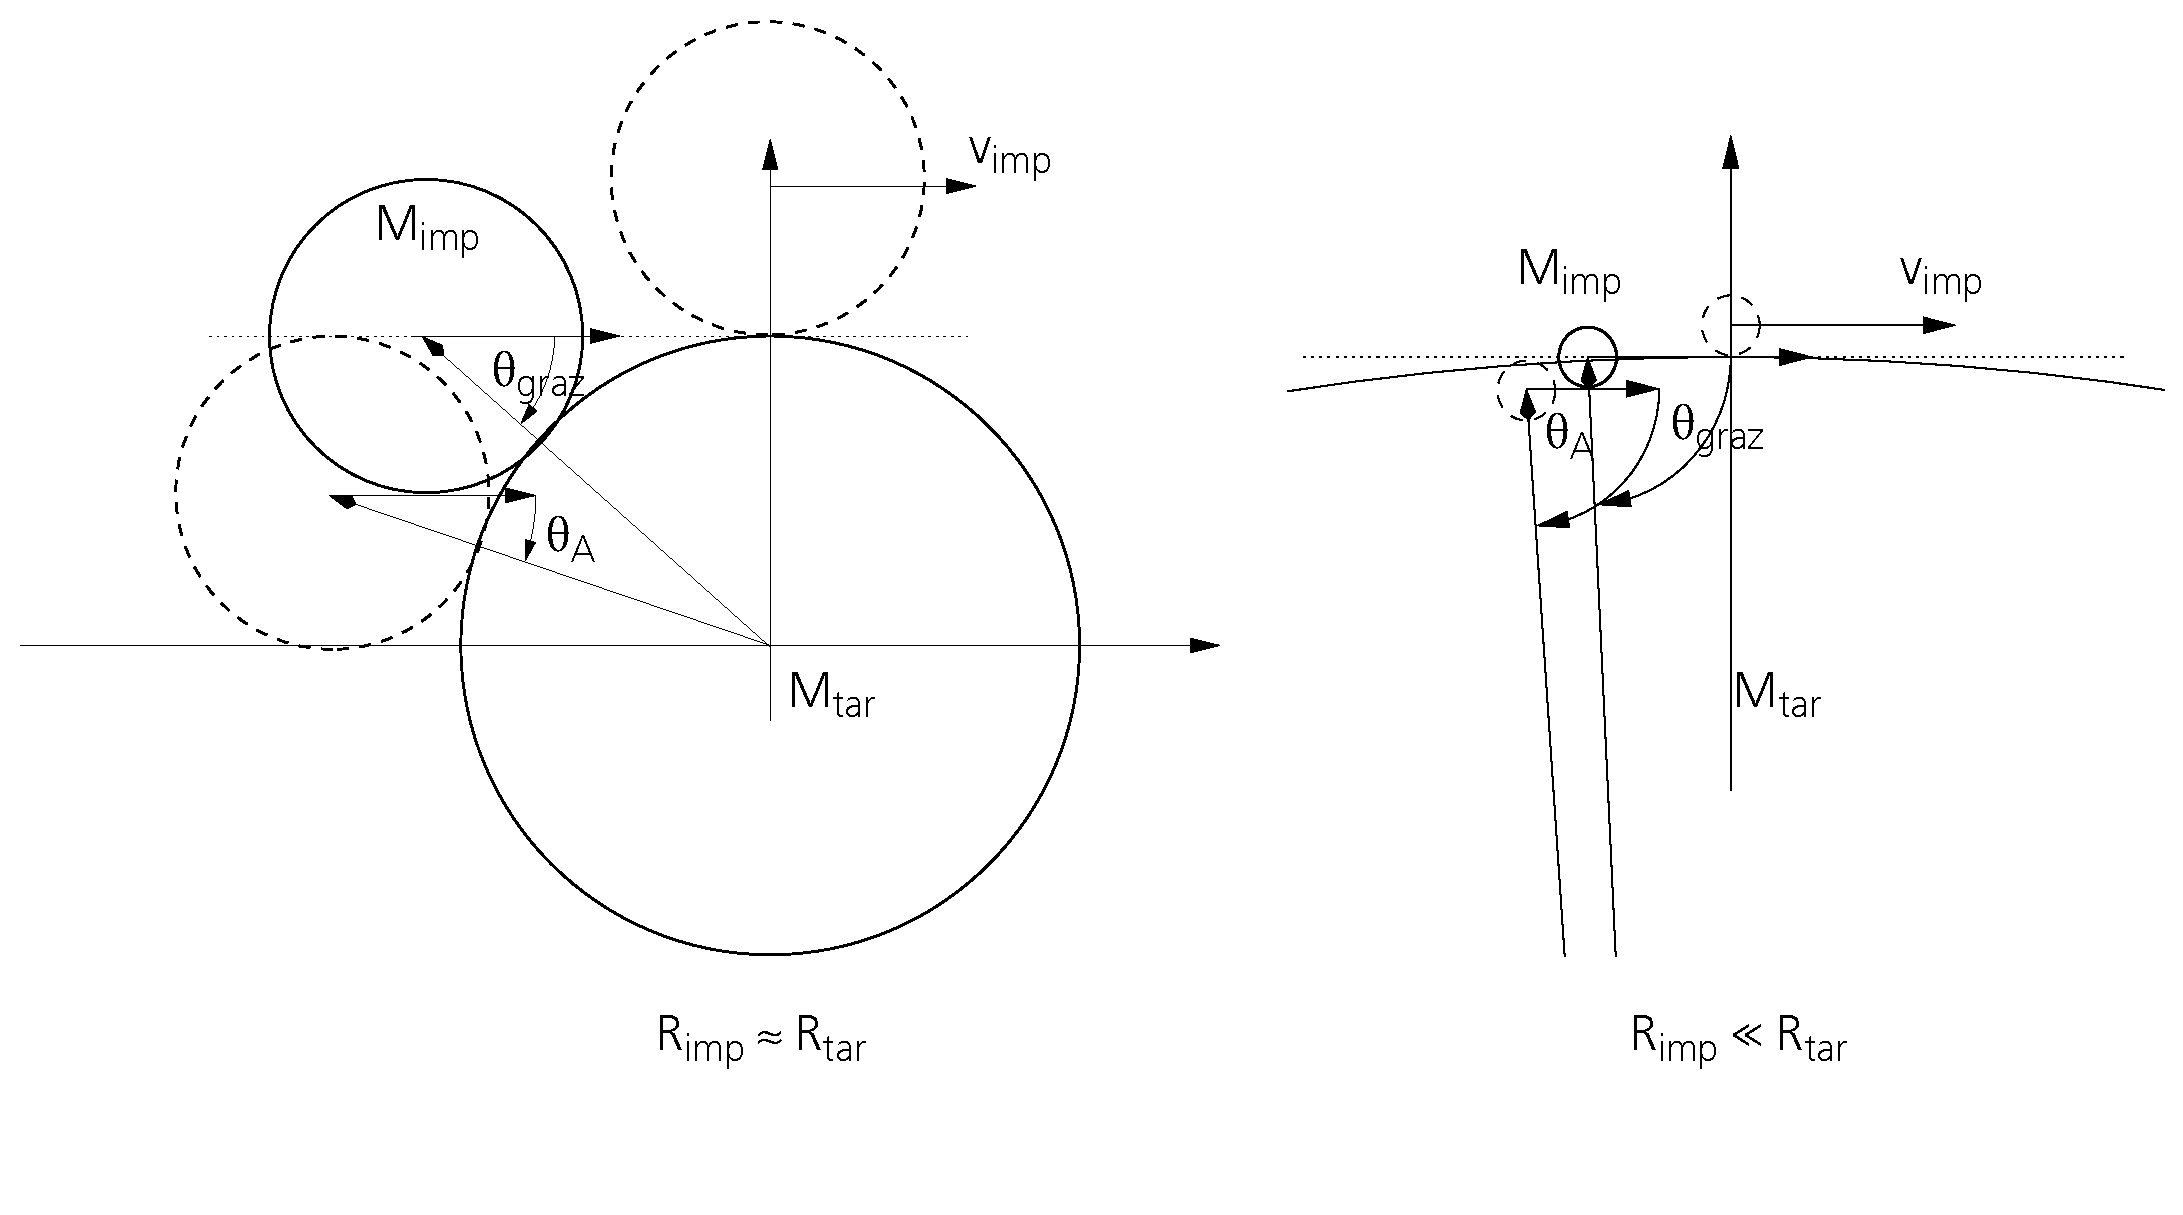
\includegraphics[scale=0.4]{03_grazing}
\caption{Impact geometry for a similar-sized collision on the left side. The right plot shows a collision between a relatively small impactor compared to the target. The grazing impact angle $\theta_{graz}$ is defined as the angle for which half of the impactor simply grazes past the target \citep{Asphaug:2010p3539}. The dashed circles show the largest impact angle for which no impactor material would graze past the target $\theta_A$ and the $90^\circ$ impact angle for which the whole impactor grazes past the target.}
\label{ch03_fig03}
\end{center}
\end{figure}

\begin{figure}
\begin{center}
\includegraphics[scale=0.7]{05_Mhit}
\caption{Relative volume of the impactor ($V_{hit, imp}$, left plots) and the target ($V_{hit, tar}$, right plots) hit by the other body as a function of impact angle (top plots) and impact parameter (bottom plots, $b = \sin \thimp$ ) for different mass ratios $\gamma$. Compare figure \ref{ch07_fig01} for an illustration of those volumes. Note that the ratio of radii scales with the cubic root of the mass ratio: $R_{imp} / R_{tar} \sim \sqrt[3]{\gamma}$. The dotted line shows for which impact angle half of the impactor volume grazes past the target. } 
\label{ch03_fig05}
\end{center}
\end{figure}

Assuming the impactor follows a straight trajectory, the volume missing the target can be calculated by integrating the cross section along the target volume (Compare appendix \ref{ch07_sec01} for the derivation). Figure \ref{ch03_fig05} on the left side shows the relative volume of the impactor missing the target ($V_{hit, imp}$) as a function of impact angle for different mass ratios $\gamma$ assuming constant and equal density spheres as bodies. The volume follows a step-function for very small impactors (small $\gamma$) with a sharp drop-off to zero near $90 \deg$. For similar-sized collisions with $\gamma = 0.1 \dots 1.0$ the relative volume smoothly increases for smaller impact angles and opens up the possibility for a variety of collisional outcomes between a total hit and a total miss. For example even for a rather small $\gamma = 0.1$, the relative volume hit by the impactor varies between 0 and 1 over an impact angle range of $30 \deg$.

Similar sized collisions are interesting, because bodies in planetary systems grow mainly by big accretionary events. Or in other words, the evolution of the largest bodies is dominated by similar-sized collisions. Many phenomena in planetary systems can best be explained as direct results of similar-sized collisions. Examples are the formation of the Earths Moon \citep{Benz:1985p1755}, Plutos companion Charon \cite{Canup:2005p1987} or also the anomalously high density of Mercury \cite{Benz:1988p3336}. Understanding similar-sized collisions is therefore key for understanding planet formation in general.

Compared to cratering collisions the interplay of the governing physics in similar-sized collisions with impact velocities on the order of the mutual escape velocity the target and the impactor is more complex and there are only very basic scaling laws predicting the outcomes of similar-sized collisions. Hydrodynamics, gravity and thermodynamics interact in a complicated way and need to be modeled explicitly. The goal of this chapter is to perform a small parameter study in the regime of similar-sized collisions by performing a large number of impact simulations and then looking at various characteristic parameters describing the outcome of the collisions. The first section gives a quick overview of the physical processes involved in similar sized collisions and their associated timescales. In a second section, the detailed setup of the simulations and the used parameters are described. The actual results are presented in the third and summarized in the fourth section.

\section{Physics of similar-sized collisions}
Looking at the associated timescales of physics gives a feeling on what are the important aspect of physics in similar-sized collisions. In the gravity regime, where the impact velocities are on the order of the mutual escape velocity, similar-sized collisions possess the nice property of scale-invariance on the first order: When the impact velocity is scaled to the escape velocity $\vesc$ and time to the collisional time $\tcol = ( \Rimp + \Rtar ) / \vesc$ the collision becomes scale-invariant. In other words: A collision at a given impact velocity relative to the escape velocity and angle for a certain mass ration $\gamma = \Mimp / \Mtar$, has the same outcome for a target mass of $0.01 \ME$ and $1.0 \ME$ assuming the bodies have in both cases the same density and effects like shocks or compressibility can be neglected.

The collisional timescale is an estimate on how long it takes for the impactor to penetrate through the target and is given by
\begin{align}
\tau_{coll} = \frac{2 (\Rimp + \Rtar)}{\vimp} \sim \frac{\vesc}{\vimp} \frac{2 R_{tot}}{\vesc} \sim \frac{\vesc}{\vimp}  \frac{2 R_{tot}}{\sqrt{G \rho} R_{tot}} \sim \frac{\vesc}{\vimp} \frac{1}{\sqrt{\rho}}
\end{align}
where the mutual escape velocity is given by $\vesc = \sqrt{ 2 G \frac{\Mtar + \Mimp}{\Rtar + \Rimp} }$ and constant density bodies are assumed. Gravitational restitution happens on the gravitational timescale given by
\begin{align}
\tau_{grav} = \sqrt{\frac{3 \pi }{G \rho} } \sim \frac{1}{\sqrt{\rho}}
\end{align}
and is on the same order of magnitude as the collisional timescale. Both timescales depend only on the bodies density. The collisional timescale also weakly depends on the mass ratio ($\sim \sqrt[3]{\gamma}$), but stays still in the same order of magnitude for the similar sized collisions mass ratios of $\gamma = 0.1 \dots 1$. For a collisions between with $\Mimp = \Mtar = 0.1\ME$ and $\Rimp = \Rtar = 0.55 \RE$ at their mutual escape velocity, the collisional timescale yields $50$ min, whilst the gravitational timescale for a differentiated silicate and iron body with a mean-density of $4g/cm^3$ is around $100$ mins. Collisions for which the collisional timescale is on the same order of magnitude as the gravitational timescale are also called \emph{gravity dominated}, because the collision happens over a timescale in which gravity affects the whole system. If $\vimp \gg \vesc$, gravitational interacting during the collision process can be neglected and only plays a role for eventual re-accretion  of the remnants, although due to their high relative velocities the remnants will simply be dispersed.

Other physical effects are not scale-invariant, for example viscosity. \cite{Asphaug:2010p3539} argues as follows, that viscosity can be neglected in similar-sized collisions for bodies of at least a certain size: Characteristic stresses due to gravity are 
\begin{equation}
\sigma_{grav} \sim P_0 \sim G \rho^2 R^2
\end{equation}
where $P_0$ is the pressure order of magnitude inside the body with radius $R$. The strain rate $\dot{\epsilon}$ for a given Newtonian viscosity $\nu$ is then
\begin{equation}
\dot{\epsilon} = \frac{\sigma}{\nu}
\end{equation}
The strain which can develop over a gravitational timescale under viscosity is then
\begin{equation}
\epsilon = \frac{\dot{\epsilon}}{\tau_{grav}}
\end{equation}
Viscosity becomes an important effect, if the maximal strain which can develop over a gravitational timescale is only around unity. Or in other words, when the timescale for strain of the order unity becomes the same order of magnitude as the gravitational timescale, then viscosity is an important effect. Viscosity in the mantle of the early Earth was around $\nu \approx 10^9~\textrm{poise}$ \citep{2004Tectp.384...55W}, whereas for completely molten rock even lower values of around $\nu \approx 10^8~\textrm{poise}$ are expected. \cite{Asphaug:2010p3539} gives a lower limit of a few $100km$ for solid and around $10km$ for partially molten bodies for the size for which viscosity can be neglected and using a inviscid hydrodynamics solver is valid. Large bodies can be assumed to be molten during the early stages of planet formation.

Shocks are another effect where similar-sized collisions deviate from scale-invariance: The escape velocity scales $\vesc \sim M^\frac{1}{3}$ for constant density bodies \footnote{$\vesc = \sqrt[6]{8 \pi G^3 \rho} M^\frac{1}{3} \sim M^\frac{1}{3}$ for constant density sphere} and is around $1km/s$ for a density of $4g/cm^3$ and a mass of $10^{-3} \ME$. This is below the speed of sound in silicates ($\approx 3 km/s$, \cite{Melosh:2007p3502}), so that a collision with an impact velocity on the order of the escape velocity will produce acoustic waves but no strong shocks. For bodies with masses higher than a few Moon masses, the impact velocity comes into the same range as the speed of sound. Collisions are now in the hypervelocity regime and produce strong shocks, leading to a considerable heating. Figure \ref{ch03_fig06} shows the expected random velocities for a given size and eccentricities of bodies, with the speed of sound 

\begin{figure}
\begin{center}
\includegraphics[scale=0.7]{06_vimp}
\caption{An order of magnitude estimation of the random velocities for bodies undergoing collisions in a protoplanetary system with a solar mass central star. The random velocity is roughly the Kepler velocity times the orbital eccentricity. Shown are isolines of velocities for given distance from a star with a solar mass for given eccentricities. The red line shows the speed of sound of for quartz at standard conditions \cite{Melosh:2007p3502}. Note that the actual impact velocity is given by $\vimp = \sqrt{ v_{rand}^2 + \vesc^2}$ and depends on the masses of the two colliding bodies. Due to the high Kepler velocity in the inner parts of the system, even small eccentricities lead to random velocities well above the speed of sound for silicates and therefore to hypervelocity impacts even for small bodies.}
\label{ch03_fig06}
\end{center}
\end{figure}
The goal of this parameter study is now to get quantitative results for various quantities and to check whether they are scale-invariant or not.

\section{Setup and parameters used}
A similar-sized collisions encompasses many parameters, the most important ones being target mass $\Mtar$, mass ratio of the impact to the target $\gamma = \Mimp / \Mtar$, impact velocity $\vimp$ and impact angle $\thimp$. Often the scaled impact parameter $b'=\sin{\thimp}$ is alternatively used instead of the impact angle. These parameters span a 4-dimensional parameter space which will be explored in this parameter study. When using the impact angle, the four parameters have the nice property of having distinctive units, so we can write all four or a subset of them in the short form $\{\Mtar, \gamma, \thimp, \vimp\}$ with the $cgs$-units $\{[g], [1], [\deg], [cm/s]\}$.

Additional parameters are the pre-impact rotation of both the impactor and the target, which in principle spans another 6-dimensions into the parameter space. Another parameter study concerning the formation of the Earths Moon by \cite{Canup:2008p3551} analyzed the effect of pre-impact rotation of the two bodies onto disk formation after the collision and found it to be non-negligible. The composition and interior thermal profiles of both bodies are also inform parameters. They both determine the density distribution inside the bodies and therefore also the dynamics of the collision. The internal profile furthermore determines the radius of the body and therefore the impact geometry, the mutual escape velocity and accordingly the actual impact velocity. These additional parameters are not further explored in this study.

\begin{figure}
\begin{center}
\includegraphics[scale=0.7]{01_overview_params.pdf}
\caption{Overview of the sampling points in the 4-dimensional parameter space spanned by $\big\{ \Mtar, \gamma, \thimp, \vimp / \vesc \big\}$. The left plot shows the mass pairs for both bodies. Grey points denote \emph{r3} bodies (pure silicate), red points \emph{c1} bodies (chondritic, differentiated) and blue points \emph{i1} bodies (icy, differentiated). For each mass pair a total of 105 simulations sample the $\big\{ \thimp, \vimp / \vesc \big\}$ sub-space. Points in this sub-space are chosen so that regions of interest are sampled more accurately, for example in case of slow impact velocities ($\vimp < 1.5 \vesc$) and grazing impact angles ($\thimp > 45 \deg$).}
\label{ch03_fig01}
\end{center}
\end{figure}
\begin{figure}
\begin{center}
\includegraphics[scale=0.8]{07_strucs.pdf}
\caption{Isentropic internal structures of the bodies used in the simulations. The first row of plots shows the density profiles, the second row the pressure and the third row the temperatures. The first column of plots shows silicate bodies with a $100 wt\%$ $\silc$ composition with the following masses from left to right: 0.1 (blue curve), 0.2 (red), 0.5 $\ME$ (magenta). The second column shows structures of differentiated bodies of chondritic composition with a $70 wt\%$ $\silc$ mantle and a $30 wt\%$ iron core: 0.002 (red), 0.007 (green), 0.01 (blue), 0.02 (red), 0.035 (black), 0.07 (green), 0.1 (blue), 0.2 (red), 0.7 (green) and 1.0 $\ME$ (blue). The last column on the right shows a few structures with a composition typical to regions beyond the snow line with $50 wt\%$ water ice, $35 wt\%$ $\silc$ and $15 wt\%$ iron. Masses range from 0.002 (red), 0.01 (blue), 0.02 (red), 0.1 (blue), 0.2 (red) and 1.0 $\ME$ (blue) from left to right. The radius of the structures depends on the average density and therefore also on the composition of the bodies. Icy bodies have low average densities compared to chondritic bodies. Note that the bodies entirely composed of $\silc$ have a higher average density than equally massive bodies with a chondritic composition, due to the higher compressibility of $\silc$ compared to iron. In the core of the pure silicate bodies, the density reached more than twice the reference density of $\silc$, while the iron cores of the chondritic bodies is only slightly compressed.}
\label{ch03_fig07}
\end{center}
\end{figure}

The strategy for sampling the parameter space goes as follows: For three different types of body composition sets of simulations are performed. Simulation set \emph{r3} uses homogeneous bodies made up of $100 \wtp~\silc$, simulation set \emph{c1} uses differentiated bodies with a chondritic composition of $70 \wtp~\silc$ and $30 \wtp~\iron$ and simulation set \emph{i1} uses differentiated bodies with a composition typical for bodies beyond the snow line of of $50 \wtp~\watr$, $35 \wtp~\silc$ and $15 \wtp~\iron$. Figure \ref{ch03_fig07} shows the internal structures for this three different types of bodies.

The general idea now is to use the \rss simulation with its simple internal structures to get a feeling for the different collisional effects and the scaling. The more realistic \css and \iss are then used to model actual collisions in planetary systems. Figure \ref{ch03_fig01} shows the sampling of the 4-dimensional parameter space mentioned above for the three different simulation sets.  The \rss simulation set uses three different mass ratios $\gamma = \Mimp / \Mtar$ with a common impactor mass of $0.1 \ME$. The simulation sets \css and \iss cover three magnitudes of target masses in the range important for late terrestrial planet formation ($0.01 \dots 1 \ME$). The \css simulation set covers each target mass with at least impactors with a mass ratio of $\gamma = 0.2$ and  $0.7$. For the $0.1 \ME$ target, additional impacts with a mass ratio of $\gamma = 0.35$ and $0.1$ are also used. The \iss simulation set only uses impactors with a mass ratio of $\gamma = 0.2$. Figures \ref{ch03_fig29a} to \ref{ch03_fig29c} show the parameters used for each body pair in each simulation set. Note that in the \rss simulation set a few simulations have not been performed and are missing in the results. The number of particles is around $100'000$ in the target body, so that shocks are sufficiently well resolved with $\approx 50$ particles along the targets diameter.

For each $\{ \Mtar, \Mimp \}$ combination, the parameter subspace spanned by $\big\{ \thimp, \vimp / \vesc \big\}$ is sampled. Figure \ref{ch03_fig01} shows on the right plot the used data points. The distribution covers areas of interest with more data points, for example for small impact velocities ($\vimp < 1.5 \vesc$) and grazing impact angles ($\thimp > 45 \deg$). In total a 105 individual simulations are performed for each body pair. The bodies used in the simulations are prepared as described in section \ref{ch02_sec04_ss02} and set up as described in \ref{ch02_sec04_ss04}. The initial separation $r_0$ is set to $5 (\Rimp + \Rtar)$ and simulations are integrated until $50 \tau_{coll}$ after first contact of the bodies which equals to $t = 0$. This is long enough in almost any case to get converging values for the interesting quantities in collisions. Figure \ref{ch03_fig31} shows as an example various interesting quantities for the $\{0.1 \ME, 0.035 \ME, 1.60 \vesc, 38 \deg \}$ simulation in simulation set \css as a function of time. All of the quantities converge on a much smaller timescale than $50 \tau_{coll}$.
\begin{figure}
\begin{center}
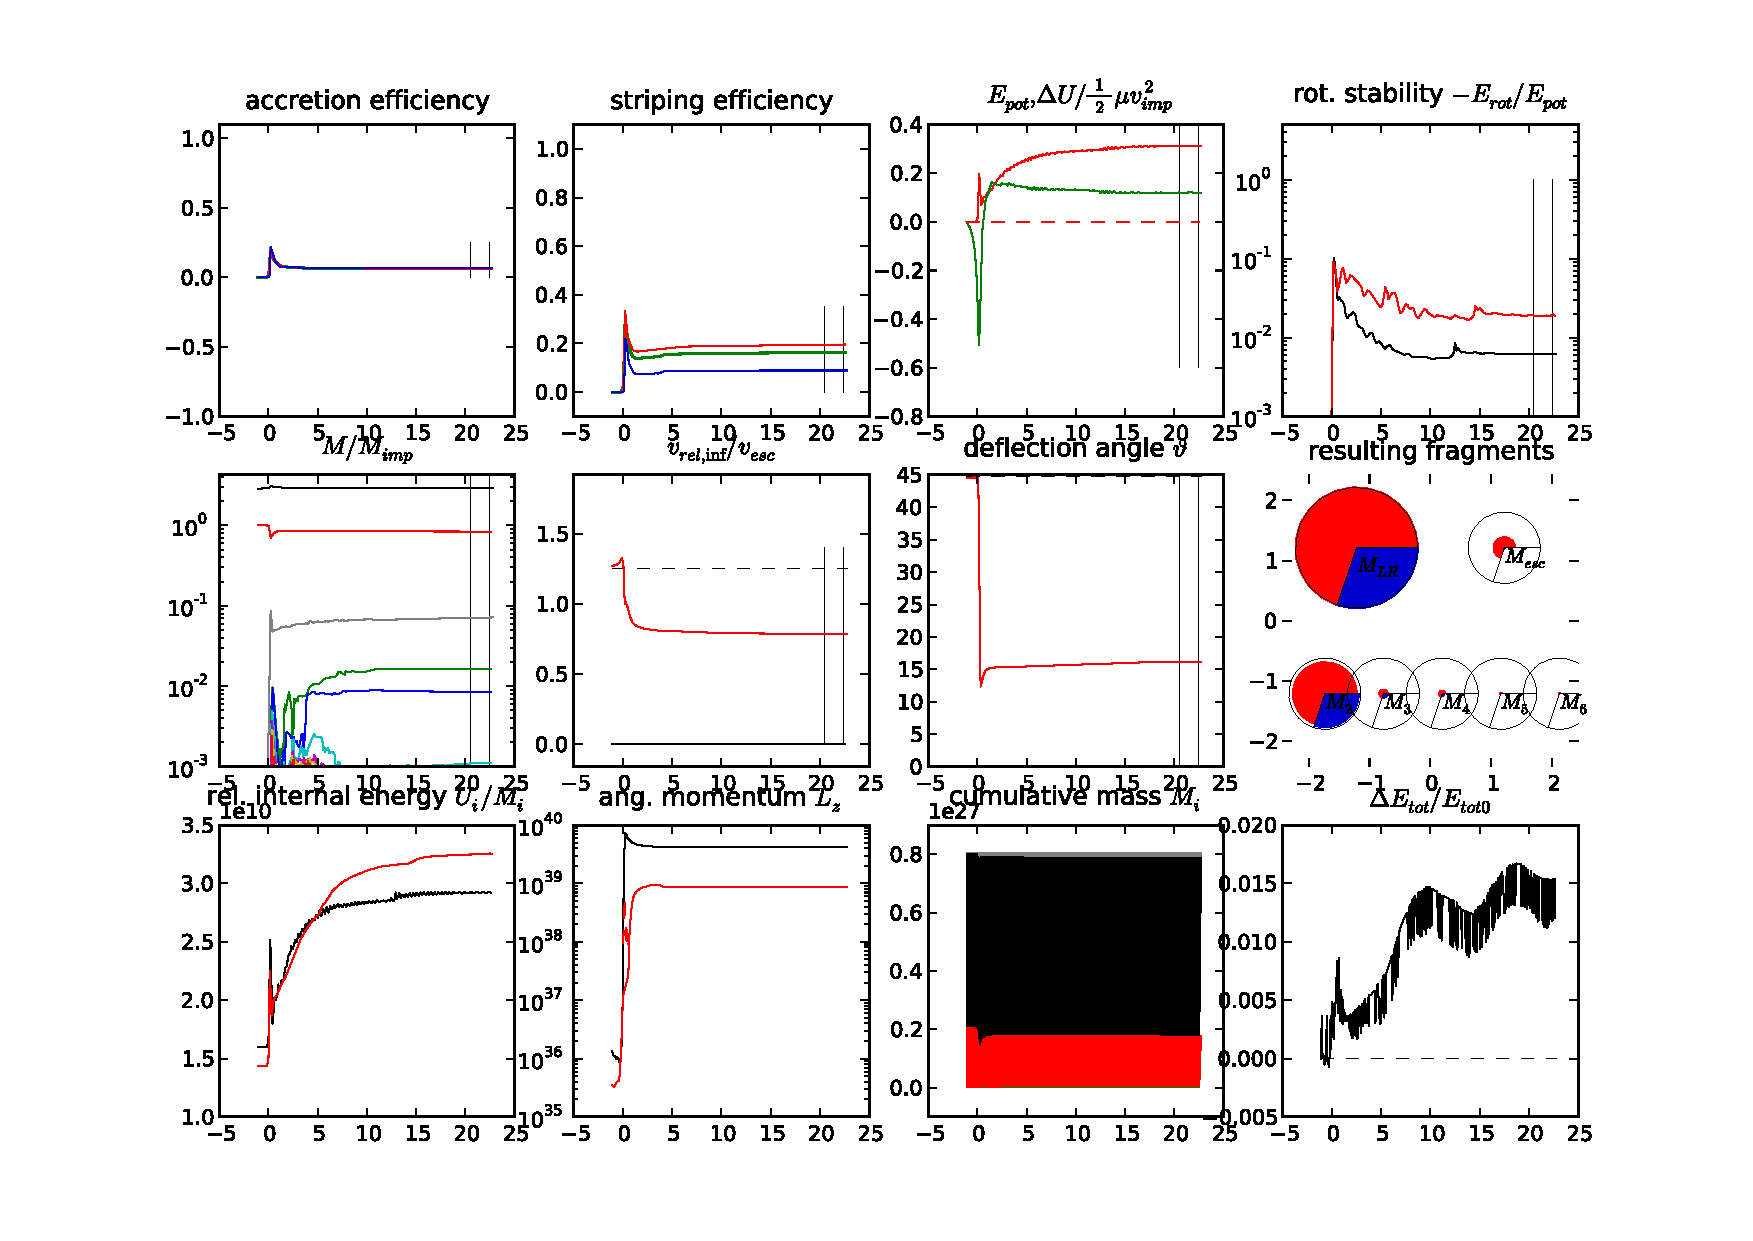
\includegraphics[scale=0.6]{31_sim_summary.pdf}
\caption{A summary for various quantities for the $\{0.1 \ME, 0.035 \ME, 1.60 \vesc, 38 \deg \}$ simulation in simulation set \css as a function of time. The x-axis in all plots denotes time in hours relative to the time of impact. One can see that all quantities converge much earlier than $50 \tau_{coll} = 22.76h$. The quantities shown in the top row are from left to right: Accretion efficiency $\xi$ (blue curve for iron, red for silicate and green for overall accretion), striping efficiency with the same color coding, change in potential (green) and internal energy (red) scaled to the reduced impact energy and finally on the far right the ratio of rotational to potential energy for the largest (black) and second remnant (red) as a measure for rotational stability. The middle row shows from the left: Remnant masses scaled to the impactor mass, relative velocity between the largest and the second remnant at infinity compared to the theoretical value expected from pure two-body interaction (dashed line), deflection angle of the second remnant compared to the theoretical two-body value (dashed line) and on the far right the composition of the remnant bodies and the ejecta. The bottom row shows from left to right: Mean specific internal energy ($erg/g$) for the largest (black) and the second remnant (red), angular momentum of the largest (black) and the second remnant (red) in $g~cm^2 / s$, mass partition into ejecta (grey), largest remnant (black), second remnant (red) and tertiary remnants (other colors). The far right shows the relative change in total energy over time as a measure for energy conservation. Errors in energy conservation mainly come from the removal of escaping particles at large distances. All the quantities will be explained below.}
\label{ch03_fig31}
\end{center}
\end{figure}
The only problematic cases where the quantities do not converge during this timescale, are when the impactor is being slowed enough to enter a closed orbit around the target with a very long orbital timescale. Such highly eccentric orbits lead to a secondary impact, where tidal effects can eject major fractions of the impactor out of the largest remnant. The orbital timescale may be $\gg 50 \tau_{coll}$, so that estimating the various quantities at that point in time leads to false results. In principle one could treat the secondary impact as a new collision scenario, but the problem is that our study does not cover impacts below the escape velocity and with impactor pre-rotation, which usually develops during the first collision. Such problematic cases occur for impact velocities slightly above the escape velocity and grazing impact angles. Figure \ref{ch03_fig30} shows such an example with the parameters $\{0.1 \ME, 0.1, 1.05 \vesc, 60 \deg \}$.
\begin{figure}
\begin{center}
\includegraphics[scale=2.0]{30_elliptic_sim_out2.png}
\includegraphics[scale=2.0]{30_elliptic_sim_out3.png}
\includegraphics[scale=2.0]{30_elliptic_sim_out4.png}
\caption{Three successive snapshots along the impact plane of simulation $\{0.1 \ME, 0.01 \ME, 1.05 \vesc, 60 \deg \}$ of simulation set \css. The impactor (orange and light blue parts) is put on a highly eccentric orbit with an orbital time much longer than $50 \tau_{coll} = 30.43h$ (last snapshot).}
\label{ch03_fig30}
\end{center}
\end{figure}

The post-processing algorithms described in sections \ref{ch02_sec04_ss05} and \ref{ch02_sec04_ss07} are run every $0.1 \tau_{coll}$ in order to get continuous evolutions of the various quantities as shown in figure \ref{ch03_fig31}. A number of python scripts is used to run a simulation set from setting up the individual simulations, running them up to cleaning up the data and storing the results for further post-processing.

\afterpage{
%\clearpage% To flush out all floats, might not be what you want
\begin{landscape}
\begin{figure}
\begin{center}
\includegraphics[scale=1.0]{29_params_r3.pdf}
\caption{Number of particles, mean density $\bar{\rho}$ and mean smoothing length $\bar{h}$ for the target and impactor bodies and $50 \tau_{coll}$ for a $\vimp = \vesc$ collision in the \rss simulation set.}
\label{ch03_fig29a}
\end{center}
\end{figure}
\begin{figure}

\begin{center}
\includegraphics[scale=1.0]{29_params_c1.pdf}
\caption{Number of particles, mean density $\bar{\rho}$ and mean smoothing length $\bar{h}$ for the target and impactor bodies and $50 \tau_{coll}$ for a $\vimp = \vesc$ collision in the \css simulation set.}
\label{ch03_fig29b}
\end{center}
\end{figure}

\begin{figure}
\begin{center}
\includegraphics[scale=1.0]{29_params_i1.pdf}
\caption{Number of particles, mean density $\bar{\rho}$ and mean smoothing length $\bar{h}$ for the target and impactor bodies and $50 \tau_{coll}$ for a $\vimp = \vesc$ collision in the \iss simulation set.}
\label{ch03_fig29c}
\end{center}
\end{figure}
\end{landscape}
}


\section{Results}
In this section we discuss several quantities which parametrize the outcome of simulated similar-sized collisions. Previous work is compared with the results of this parameter study and the differences are discussed. 
%%
% Largest remnant
%% 
\subsection{Largest remnant mass $\Mlr$, accretion efficiency $\xi$ and critical impact velocity $\vcr$}
Maybe the most important quantity of a similar-sized collisions is the mass of the largest collision remnant $\Mlr$. It is the defined as the mass of the heaviest gravitationally bound system well after the collision. Note that this is not always just one body. Part of the largest remnant may also be satellites in stable orbits around the largest fragment. For example the Earth-Moon system is considered to be one single largest remnant of the giant impact. While most of the mass of the largest remnant naturally comes from the collision target, it can either accrete mass from the impactor or in high-energy events loose mass through erosion. A useful parameter related to $\Mlr$ is the accretion efficiency
\begin{equation}
\xi = \frac{\Mlr - \Mtar}{\Mimp}
\end{equation}
which gives the change in mass from the target to the largest remnant normalized to the impactor mass $\Mimp$. If the impactor is accreted perfectly $\xi = 1$, if no mass is accreted or lost $\xi = 0$ and in case of target erosion where the target looses mass $\xi < 0$.

Figures \ref{ch03_fig08a} to \ref{ch03_fig08c} give the accretion efficiency for the three simulation sets as a function of the impact angle $\thimp$ for different impact velocities. For all three types of bodies and all mass ratios, the same characteristics can be observed: For very slow impact velocities of $\vimp = 1.00 \dots 1.05 \vesc$ (red and orange curves, x marker), the impactor is fully accreted independent of the impact angle. For very grazing impact angles a small fraction of the impactor is accelerated above escape velocity and escapes the remnant, so that the accretion efficiency is slightly below 1. This effect can be seen for $\thimp > 60 \deg$, especially for the $1.05 \vesc$ cases. A slight increase in impact velocity to $1.10 \vesc$ (green curve, x marker) lets the impactor miss the target almost unaltered if the impact angle is above a critical value, which seems to be mainly dependent on the mass ratio $\gamma$. Independent of type of body or the magnitude of the targets mass, this critical angle is between $60 \dots 75 \deg$ for $\gamma = 0.7$,  around $60 \deg$ for $\gamma = 0.2$ and slightly below $60 \deg$ for $\gamma = 0.1$. Above this critical angle, $\xi$ goes almost to 0. This is consistent with the results from \cite{Agnor:2004p3329} (compare figure 1) which finds a critical angle above $60 \deg$ for $\gamma = 1.0$. Additional simulations with $\gamma = 0.1$ and $0.5$ shown in figure 8 of \cite{Asphaug:2010p3539} also yield critical impact angles consistent with the results of this study (for a conversion between the relative velocity between the impactor and target at infinity $\vneginf$ and $\vimp$ check table \ref{ch03_tbl01}).
\begin{table}[htdp]
\begin{center}
\begin{tabular}{l|r|r|r|r|r|r|r|r}
$\vimp / \vesc$ & 1.00 & 1.05 & 1.10 & 1.15 & 1.20 & 1.30 & 1.40 & 1.50 \\
\hline
$\vneginf / \vesc$ & 0.00 & 0.32 & 0.46 & 0.57 & 0.66 & 0.83 & 0.98 & 1.12\\
\hline
\hline
$\vimp / \vesc$ & 1.60 & 1.70 & 1.80 & 2.00 & 2.50 & 3.00 & 3.50 & 4.00\\
\hline
$\vneginf / \vesc$ & 1.25 & 1.37 & 1.50 & 1.73 & 2.29 & 2.83 & 3.35 & 3.87\\
\end{tabular}
\end{center}
\caption{Conversion table $\vneginf \leftrightarrow \vesc$ based on the simple energy budget $\vimp^2 = \vneginf^2 + \vesc^2$.}
\label{ch03_tbl01}
\end{table} 
Further increasing the impact velocity ($> 1.10 \vesc$) shifts this critical angle to smaller values and transforms the abrupt change from $\xi \approx 1$ to $\xi \approx 0$ into a smoother transition over a larger span of impact angle. For small mass ratios like $\gamma = 0.1$ in the \css or the simulation set or the $\gamma = 0.1$ and $0.2$ simulations in set \rss, the accretion efficiency follows a curve similar to the relative volume of the impactor hitting the target (black dashed line in all figures \ref{ch03_fig08a} to \ref{ch03_fig08c}). The impact velocity where the two quantities correlate best is between $1.20 \dots 1.40 \vesc$. The reason why this correlation gets weaker for higher mass ratios, is because the simple volumetric guess assumes that the target is not changed considerably and simply cuts through the impactor. The alteration of the target increases with higher mass ratios and the model breaks down. Another complication is that equating the cross-section volume with the accreted mass only works for constant-density bodies. While this is roughly the case in simulation set \rss with its pure silicate bodies, this assumption breaks down in \css and \iss, where the heavier cores carry more kinetic energy per volume than the mantle material. In this case it makes a difference whether the core misses or hits the target. 

By further increasing the impact velocity, the accretion efficiency goes  $\xi < 1$ even for $0 \deg$ head-on impacts. For high enough velocities it becomes negative and the target is being eroded. While for hight impact velocities $\vesc > 3.00 \vesc$, the accretion efficiency becomes smaller for smaller impact angle, the effect reverses in an regime between $2.00 \dots 3.00 \vesc$, where the accretion efficiency actually increases again between for decreasing impact angles between $0 \dots 20 \deg$. This can be explained due to the fact that for a more head-on collision distributes the impact more evenly among the target, so that less mass reaches the required kinetic energy to leave the largest remnant. This effect is more prominent in the simulation sets with differentiated bodies (\css and \iss).

The results for the accretion efficiency are in agreement with previous work. \cite{Benz:1988p3336} performed SPH collision simulations with $\Mtar = 0.124 \ME$, $\gamma = 1/6$, $\vimp = 2.2 \dots 8.46 \vesc$ and $\thimp = 0 \dots 32 \deg$. Runs $9 \dots 11$ are comparable with simulations performed in this study. While we have no data for $\Mtar = 0.124 \ME$ and $\gamma = 1/6$, the results should lie somewhere in between the runs for $\Mtar = 0.1 \ME$ and $\gamma = 0.1$ and $0.2$. Run 9 in  \cite{Benz:1988p3336} with $\{0 \deg, 3.34 \vesc \}$ obtained a $\gamma = -2.14$, in accordance with $\xi = -1.82$ for our simulation with $\{0.1 \ME, 0.1, 0 \deg, 3.50 \vesc \}$ and $\xi = -1.70$ for $\{0.1 \ME, 0.2, 0 \deg, 3.50 \vesc \}$. Run 10 with the parameters $\{ 0 \deg, 2.23 \vesc \}$ obtains $\xi = -0.14$ and lies in between $\xi = 0.48$ for our simulation $\{0.1 \ME, 0.2, 0 \deg, 2.50 \vesc \}$ and $\xi = -0.19$ for $\{0.1 \ME, 0.2, 0 \deg, 2.50 \vesc \}$. Run 11 uses a larger impcat angle with the parameters $\{ 32 \deg, 3.34 \vesc \}$ and yields $\xi = -1.12$, comparable with $\xi = -0.76$ of simulation $\{0.1 \ME, 0.1, 30 \deg, 3.50 \vesc \}$ and $\xi = -0.58$ of simulation $\{0.1 \ME, 0.2, 30 \deg, 3.50 \vesc \}$. The differences in the results between our simulations and  \cite{Benz:1988p3336}  are most probably due to the much lower resolution ($4k$ vs. $110k - 120k$ particles) and to the different version of ANEOS (dunite without molecules vs. $\silc$ with molecules).

\afterpage{
%\clearpage% To flush out all floats, might not be what you want
\begin{landscape}

\begin{figure}
\begin{center}
\includegraphics[scale=1.0]{08_accreff_r3.pdf}
\caption{Accretion efficiency $\xi$ as a function of the impact angle for different relative impact velocities. Each subplot shows a set of simulations for a given target mass $\Mtar$ and mass ratio $\gamma = \Mimp / \Mtar$. Each point shows the outcome of an individual simulation of the \emph{r3} simulation set involving bodies composed purely of $\silc$. The black dashed line shows the relative volume of the impactor hitting the target for the given mass ratio (compare figure \ref{ch03_fig05}).}
\label{ch03_fig08a}
\end{center}
\end{figure}

\begin{figure}
\begin{center}
\includegraphics[scale=1.0]{08_accreff_c1.pdf}
\caption{Accretion efficiency $\xi$ for the \emph{r3} simulation set with bodies of chondritic composition (compare figure \ref{ch03_fig08a}. Each row shows a different magnitude of target mass, each column a different mass ratio.}
\label{ch03_fig08b}
\end{center}
\end{figure}

\begin{figure}
\begin{center}
\includegraphics[scale=1.0]{08_accreff_i1.pdf}
\caption{Accretion efficiency $\xi$ for the \emph{i1} simulation set with bodies of icy composition (compare figure \ref{ch03_fig08b}).}
\label{ch03_fig08c}
\end{center}
\end{figure}

\end{landscape}
}

Figures \ref{ch03_fig09a} to \ref{ch03_fig09c} show the accretion efficiency as a function of the impact velocity for different impact angles. All mass ratios in all simulation sets show the same characteristics: For grazing impact angles ($\thimp \gg \theta_{graz}$, compare figure \ref{ch03_fig03}), the accretion efficiency is a step function of the impact velocity. Either the impactor is almost perfectly accreted or misses the target completely. Target erosion is almost negligible, even for very high impact energies. For smaller impact angles the function then transitions towards a parabolic function. Escaping mass from the largest remnant is the proportional to the impact energy or the impact velocity squared. 

This step-function property of the accretion efficiency induces the notion of categorizing the collisions. \cite{Asphaug:2010p3539} names four main categories: Slow collisions lead to an \emph{efficient accretion} ($\xi \approx 1$) of the impactor onto the target. For higher impact velocities only \emph{partial accretion} is accomplished where $0 < \xi <1$, depending on the impact angle. Another distinct regime are \emph{hit \& run} collisions \citep{Asphaug:2006p3729} for which $\xi \approx 0$ and where the targets mass remains practically unaltered. Nevertheless such collisions are interesting, because the impactor might still undergo modifications like spinning up or loosing mass. The fourth regime is \emph{erosion and disruption} for which $\xi < 0$.

\cite{2010ApJ...714L..21K} performed a similar parameter study and extracted as a characteristic quantitiy the critical impact velocity $v_{cr}$ for which
\begin{equation}
\xi(v_{cr}, \thimp, \Mtar, \Mimp) \doteq 0
\end{equation}
the accretion efficiency becomes zero as a function of impact angle, target and impactor mass. They performed SPH collision simulations with mass rations of $\gamma =$ 1.0, 0.66, 0.50, 0.33, 0.25, 0.17, 0.11 and $M_{tot} = \Mimp + \Mtar = 0.2 \dots 2.0 \ME$ at impact velocities between $\vimp = 1.0 \dots 3.0 \vesc$ at angles between $\thimp = 0 \dots 75 \deg$. Instead of the ANEOS equation of state used here, they used the Tillotson equation of state \cite{Melosh:1989p996} which does not include phase transitions for melting or vaporization. Both the target and the impactor are differentiated bodies with $70 \wtp~\silc$ and $30 \wtp~\iron$ as in our \css simulation set. They found the following empiric fitting function for
\begin{equation}
\label{ch03_eq002}
\vcr / \vimp = c_1 \Bigg( \frac{\Mtar - \Mimp}{\Mtar + \Mimp} \Bigg)^2 \big( 1 - \sin{\thimp} \big)^\frac{5}{2} + c_2 \Bigg( \frac{\Mtar - \Mimp}{\Mtar + \Mimp} \Bigg)^2 + c_3 \big( 1 - \sin{\thimp} \big)^\frac{5}{2}  + c_4
\end{equation}
with $c_1 = 2.43, c_2 = - 0.0408, c_3 = 1.86$ and $c_4 = 1.08$. The vertical lines in figures \ref{ch03_fig09a} to \ref{ch03_fig09c} show the predicted value for $\vcr$ for each mass ratio, target mass and impact angle. Our results in simulation set \css (\ref{ch03_fig09b}) match the predicted values quite well for $\thimp \ge 20 \deg$ and $\gamma \ge 0.2$. For $\thimp < 20 \deg$ equation \ref{ch03_eq002} predicts a strong increase in $\vcr$ for small decreases in impact angle, for example for $\gamma = 0.7$ an $\vcr$ increase of over 50 \% from $\thimp = 15 \deg$ to $0 \deg$. Although our results also show a small increase in the impact velocity for which $\xi = 0$ for decreases in impact angle at already small values, but it is not as large as in the empirical function from above. The main difference between the simulations presented here and the ones from \cite{2010ApJ...714L..21K} is the equation of state or particularly the lack of proper modeling of phase changes in the Tillotson equation of state. The amount of vaporization depends strongly on the impact regime. For gravity dominated collisions in the lunar mass regime ($\Mtar \approx 0.01 \ME$), only weak shocks and therefore no significant melting or vapor production occurs. But with target masses in the order of the Earths mass, a significant amount of silicate can be vaporized, due to impact velocities above the speed of sound of silicates and the associated production of strong shocks. If the difference in the equation of state would be the cause of the disagreement of the critical velocities obtained from our results and the ones from the empiric law above, then our results should show a significant scale-dependence for the accretion efficiency. This is not the case. For a given mass range in a simulation set, the accretion efficiency is relatively scale-independent. The disagreement can best be explained by a bad fit of equation \ref{ch03_eq002} with simulation results for small impact angles in general, probably also the ones from \cite{2010ApJ...714L..21K}. For very grazing angles equation \ref{ch03_eq002} predicts slightly too slow critical impact velocities, especially for small mass ratios. For instance at $\thimp = 45 \deg$ for $\{ \Mtar = 0.1 \ME, \gamma = 0.1\}$ the accretion efficiency yields $\xi \approx 0.8$ at the predicted critical impact velocity.

The simulation sets \iss and \rss with differently composed bodies show similar results for the critical velocity and therefore are also fit equation \ref{ch03_eq002} equally well as in the \css simulation set. \cite{2010ApJ...714L..21K} use equation \ref{ch03_eq002} to determine, whether collisions in terrestrial planet formation simulations are accreting or eroding mass on the target. Considering the disagreement between the fitting function and the simulation results suggest, that expression \ref{ch03_eq002} should not be used for $\thimp < 20 \deg$ and very high impact velocities, otherwise disruptive events while be falsely treated as accretionary.

\afterpage{
%\clearpage% To flush out all floats, might not be what you want
\begin{landscape}
\begin{figure}
\begin{center}
\includegraphics[scale=1.0]{09_accreff_vimp_r3.pdf}
\caption{Accretion efficiency $\xi$ for the \emph{r3} simulation set as a function of impact velocity $\vimp$ for different impact angles. The vertical lines shows the predicted values from \cite{2010ApJ...714L..21K} for the critical impact velocity $v_{cr}$, where $\xi$ becomes negative and the target no longer accretes material but is eroded.}
\label{ch03_fig09a}
\end{center}
\end{figure}

\begin{figure}
\begin{center}
\includegraphics[scale=1.0]{09_accreff_vimp_c1.pdf}
\caption{Accretion efficiency $\xi$ as a function of impact velocity $\vimp$ for different impact angles as in figure \ref{ch03_fig09a} for the \emph{c1} simulation set.}
\label{ch03_fig09b}
\end{center}
\end{figure}

\begin{figure}
\begin{center}
\includegraphics[scale=1.0]{09_accreff_vimp_i1.pdf}
\caption{Accretion efficiency $\xi$ as a function of impact velocity $\vimp$ for different impact angles as in figure \ref{ch03_fig09a} for the \emph{i1} simulation set.}
\label{ch03_fig09c}
\end{center}
\end{figure}
\end{landscape}
}

\subsection{Catastrophic disruption threshold $Q^*_D$ and $Q^*_{RD}$}
Another quantity associated with the largest remnant is the specific impact energy required for catastrophic disruption, which is defined as a collision where the largest remnant is no more than half of the targets mass. The specific impact energy in its original definition \cite{Benz1999Icar..142....5B} is the kinetic energy of the impactor 
\begin{equation}
Q = \frac{ \frac{1}{2} \vimp^2 \Mimp }{\Mtar} 
\end{equation}
The specific impact energy required for catastrophic disruption is denoted $Q^*_D$ and fulfills
\begin{equation}
\Mlr(Q^*_D) = 0.5 \Mtar
\end{equation}
More recent work \citep{Stewart:2009p3265, 2009ApJ...700L.118M, 2010ApJ...712L..73M, Leinhardt:2011p4060} considers the reduced mass and defines the specific reduced impact energy 
\begin{equation}
\label{ch03_eq005}
Q_R = \frac{ \frac{1}{2} \vimp^2 \mu }{\Mtar + \Mimp} \hspace{2.0cm} \mu = \frac{\Mtar \Mimp}{\Mtar + \Mimp} 
\end{equation}
and defines catastrophic disruption as a collision where the largest remnant has no more than half of the total mass $\Mtot = \Mtar + \Mimp$ with the reduced catastrophic disruption threshold $Q^*_{RD}$
\begin{equation}
\Mlr(Q^*_{RD}) = 0.5 \Mtot
\end{equation}
\cite{Stewart:2009p3265} propose the simple linear relationship between the largest remnant mass and $Q_R$
\begin{equation}
\label{ch03_eq003}
\Mlr / \Mtot = - 0.5 ( Q_R / Q^*_{RD} - 1 ) + 0.5
\end{equation}
$Q^*_{RD}$ is a constant depending on the material and scale-dependent physics. A velocity dependent form for this constant in \emph{cgs}-units is given by
\begin{equation}
\label{ch03_eq004}
Q^*_{RD} = \underbrace{ q_s R^{9\mu/(3-2\phi)}_{C1} \vimp^{2-3\mu} }_{\textrm{strength regime} } + \underbrace{ q_g R^{3 \mu}_{C1} \vimp^{2-3\mu}}_{\textrm{gravity regime}}
\end{equation}
where $R_{C1}$ is the radius of a body with mass $\Mtot$ and a density of $1 g/cm^3$. The first part comes from the required energy to overcome material strength, while the second part accounts for the gravitational binding energy. For small, solid bodies ($R < 1km$), the strength term is dominating, while it becomes negligible for large bodies ($R > 100km$). For the constants, \cite{Stewart:2009p3265} find the following constants for the basalt bodies in \cite{Benz1999Icar..142....5B}: $\mu = 0.5, \phi = 8, q_s = 7 \times 10^4, q_g = 10^{-4}$. In the gravity regime, \cite{2010ApJ...712L..73M} uses the same constant but changes $\mu = 0.4$. Obviously equation \ref{ch03_eq003} does not account for the collision geometry imposed by the impact angle and therefore deviations are expected. \cite{Stewart:2009p3265} state that the relationship \emph{does not hold for conditions that depart from the catastrophic disruption regime}. This excludes explicitly collisions which are merging ($\xi \approx 1$) or collisions in the super-catastrophic regime ($Q_R / Q^*_{RD} > 2$). Note also that the predicted $\Mlr / \Mtot$ is not scale invariant, as $Q^*_{RD}$ depends on the absolute velocity.

Figures \ref{ch03_fig15a} to \ref{ch03_fig15c} show the mass of the largest remnant relative to the total mass as a function of $Q_R / Q^*_{RD}$ for different impact angles. The dashed line shows the linear relationship \ref{ch03_eq003} which is supposed to match the results. As our simulations covered the same range of impact velocities for all mass ratios, the range of $Q_R$ covered is smaller for small mass ratios. For a small mass ratio, the impact velocity needs to be higher to reach the same value of $Q_R$ than for a collision with a larger mass ratio. As expected the value for $\Mlr / \Mtot$ does not match the linear relationship for collisions at the minimal specific impact energy $Q_{R,min} = \frac{ \frac{1}{2} \vesc^2 \mu}{\Mtot}$ which are perfectly accreting for all impact angles and therefore $\Mlr = \Mtot$. 

For larger values of $Q_R$ collisions become eroding and the relationship presents a reasonable fit for the determined largest remnant masses. The fit becomes better for small mass ratios. The concept of relating the largest remnant mass with the specific impact is based on the assumption, that the impact energy is perfectly coupled into the combined mass and can be used to overcome strength and the gravitational binding energy. But for impact angles above the grazing angle, considerable mass of the impactor misses the target and part of the impact energy can not be used erode the target. This effect can be seen in the results for simulations with impact angles near or above the grazing angle. For very head-on impact angles, the relationship surprisingly also shows an inferior agreement, despite the fact that the impact energy is coupled perfectly into the combined mass. In all simulations, the $\Mlr / \Mtot$ decreases faster than linear for $\thimp < 20 \deg$. For small mass ratios ($\gamma = 0.35, 0.2, 0.1$), the impact angle for which the results match the prediction best is between $\thimp = 22 \dots 30 \deg$. For the larger mass ratios of $\gamma = 0.5$ and $0.7$, the slope of $\Mlr / \Mtot$ is best matched for $\thimp = 22 \deg$ for $Q_R > 0.5 Q^*_{RD}$ , but has quite a large offset. For smaller $Q_r$, small impact angles present a better match, but show a non-linear slope as for the small mass ratios. Nevertheless, the relationship \ref{ch03_eq003} predicts the largest remnant mass within a factor of 2 for all cases and much better for most eroding cases, which is in accordance with \cite{2009ApJ...700L.118M}. As the accretion efficiency $\xi$ above, the agreement of the relationship with the results is basically scale-invariant. The differences between different mass regimes show no systematic differences.

\afterpage{
%\clearpage% To flush out all floats, might not be what you want
\begin{landscape}
\begin{figure}
\begin{center}
\includegraphics[scale=1.0]{15_QQRD_r3.pdf}
\caption{Scaled largest remnant masses $\Mlr / M_{tot}$ as a function of the relative specific impact energy $Q_R / Q^*_{RD}$ as defined in \cite{Stewart:2009p3265} and using the parameters for $Q^*_{RD}$ as in \cite{2010ApJ...712L..73M}. The coloured lines solid lines show the simulation values for the \emph{r3} simulation set and the dashed black line shows the predicted value from the scaling law.}
\label{ch03_fig15a}
\end{center}
\end{figure}

\begin{figure}
\begin{center}
\includegraphics[scale=1.0]{15_QQRD_c1.pdf}
\caption{Scaled largest remnant masses $\Mlr / M_{tot}$ as a function of the relative specific impact energy $Q_R / Q^*_{RD}$ as in figure \ref{ch03_fig15a}, but for the \emph{c1} simulation set.}
\label{ch03_fig15b}
\end{center}
\end{figure}

\begin{figure}
\begin{center}
\includegraphics[scale=1.0]{15_QQRD_i1.pdf}
\caption{Scaled largest remnant masses $\Mlr / M_{tot}$ as a function of the relative specific impact energy $Q_R / Q^*_{RD}$ as in figure \ref{ch03_fig15a}, but for the \emph{i1} simulation set.}
\label{ch03_fig15c}
\end{center}
\end{figure}
\end{landscape}
}


%%
% second remnant 
%% 
\subsection{Second remnant mass $\Msr$}
In most collisions, the largest remnant is mainly composed from the target. Similarly, the impactor can form a second remnant in case it is not completely accreted during the collision. Figures \ref{ch03_fig26a} to \ref{ch03_fig26c} shows the second remnant masses relative to the impactor mass as a function of the impact velocity, similar to figure 15 in \cite{Asphaug:2010p3539} which shows results from the parameter study by \cite{Agnor:2004p3329}. Although his results $\gamma = 1.0$ cannot be directly compared with our $\gamma = 0.1 \dots 0.7$, the overall characteristics match well our results. For the efficiently accreting collisions with small impact velocities ($\vneginf \lessapprox 0.5 \vesc$), no second remnant is left after the collision. For higher velocities the impactor either completely or partly misses the target and a gravitationally bound second largest remnant can form. The larger the impact angle, the lower the velocity required to form a second remnant and the steeper is the increase to maximal reached mass for a given impact angle. From the maximum, the mass decreases again parabolically as a function of velocity or linearly to impact energy. The second remnant mass appears to be scale-free, but depends on the mass ratio. While for example for $\gamma = 0.7$, the impactor retains its mass entirely and becomes a second remnant with $\Msr / \Mimp \approx 1$ for angles up to $45 \deg$, the impactor looses considerably mass for low mass ratios (e.g. $\gamma = 1$) already for $\thimp < 60 \deg$. For high velocities and small angles, the second remnant mass becomes scale-dependent: For example in simulation set \css with parameters $\{0.2, \thimp < 35 \deg, 1.0 \vesc < \vneginf < 3.0 \vesc \}$, the second remnant mass decreases for larger mass regimes. While a  second remnant survives the collision for $\{0.01 \ME, 0.2, \thimp > 15 \deg, 1.0 \vesc < \vneginf < 3.0 \vesc \}$ with considerable mass between $0.1 \dots 0.5 \Mimp$, no second remnant is left over for comparable parameters but with $\Mtar = 1.0 \ME$. This can be explained, by disruption of the second remnant due to the much higher impact velocity in the $\Mtar = 1.0 \ME$ case in absolute numbers. The impact velocity is super-sonic and the second remnant is disrupted. The same effect can also be observed by comparing the three different target mass regimes in simulation set \iss.

\afterpage{
%\clearpage% To flush out all floats, might not be what you want
\begin{landscape}
\begin{figure}
\begin{center}
\includegraphics[scale=1.0]{26_SR_M_r3.pdf}
\caption{Second remnant mass $\Msr$ as a function of relative velocity at infinity before impact $v_{-\infty} / \vesc$ for the \emph{r3} simulation set. Simulations with a second remnant below 5\% of the impactors mass are not shown.}
\label{ch03_fig26a}
\end{center}
\end{figure}

\begin{figure}
\begin{center}
\includegraphics[scale=1.0]{26_SR_M_c1.pdf}
\caption{Second remnant mass $\Msr$ as a function of relative velocity at infinity before impact $v_{-\infty} / \vesc$ as in figure \ref{ch03_fig26a} but for the \emph{c1} simulation set.}
\label{ch03_fig26b}
\end{center}
\end{figure}

\begin{figure}
\begin{center}
\includegraphics[scale=1.0]{26_SR_M_i1.pdf}
\caption{Second remnant mass $\Msr$ as a function of relative velocity at infinity before impact $v_{-\infty} / \vesc$ as in figure \ref{ch03_fig26a} but for the \emph{i1} simulation set.}
\label{ch03_fig26c}
\end{center}
\end{figure}
\end{landscape}
}

Figures \ref{ch03_fig40a} to \ref{ch03_fig40c} show again the second remnant mass, but this time as a function of impact angle. For high enough impact velocities, the fit with the relative impactor volume hit by the target assuming a straight trajectory $V_{hit, imp}$ becomes obvious for simulation set \rss (figure \ref{ch03_fig40a}). The relationship holds for $\vimp > 1.10 \dots 1.15 \vesc$. For this homogenous bodies, the impactor mass hit by the target is proportional to the volume. The fit becomes a bit worse for the differentiated bodies with non-trivial structures, as can be seen with the plots for simulation set \css in figure \ref{ch03_fig40b}. The second remnant mass curves start to fit the relative hit volume for $\vimp > 1.30 \dots 1.40 \vesc$. The curve is a steeper function of the impact angle, which can be explained by considering the density profiles of the impactor bodies. In case only a very small fraction of the impactor is hit by the target, mainly low density mantle material will be abraded. So less mass is lost compared to a constant-density body with the same volume. For an impact angle near $\thgraz$, the high density core will also be affected and a small change in impact angle makes a big difference in the mass loss the impactor experiences.

\afterpage{
%\clearpage% To flush out all floats, might not be what you want
\begin{landscape}
\begin{figure}
\begin{center}
\includegraphics[scale=1.0]{40_SR_M_impa_r3.pdf}
\caption{Second remnant mass $\Msr$ as a function of impact angle for the \rss simulation set. Simulations with a second remnant below 5\% of the impactors mass are not shown. The black dashed line shows the relative volume of the impactor hitting the target $V_{hit, imp}$ (compare figure \ref{ch03_fig05}).}
\label{ch03_fig40a}
\end{center}
\end{figure}

\begin{figure}
\begin{center}
\includegraphics[scale=1.0]{40_SR_M_impa_c1.pdf}
\caption{Second remnant mass $\Msr$ as a function of impact angle as in figure \ref{ch03_fig40a}, but for the \css simulation set.}
\label{ch03_fig40b}
\end{center}
\end{figure}

\begin{figure}
\begin{center}
\includegraphics[scale=1.0]{40_SR_M_impa_i1.pdf}
\caption{Second remnant mass $\Msr$ as a function of impact angle as in figure \ref{ch03_fig40a}, but for the \iss simulation set.}
\label{ch03_fig40c}
\end{center}
\end{figure}
\end{landscape}
}

Comparing the two ratios $\Mlr / \Mtar$ and $\Msr / \Mimp$ shows an interesting property of similar-sized collisions: The smaller the mass ratio, the bigger the relative change to the impactor compared to the target. While for small ratios it requires a very high specific impact energy for the impactor to alter the mass of the target considerable, the impactor itself is altered easily ranging from complete accretion up to keeping its entire mass. This impactor perspective is an interesting aspect for planet formation models, as largest bodies in a planetary system might act as \emph{catalysts} altering a class of \emph{next-largest bodies} \citep{Asphaug:2010p3539} considerably.

A probably trivial but nevertheless important property of the second remnant mass is, that it is never larger than the impactor mass. So mass transfer during a collisions always goes from the lighter impactor to the heavier target. This is simply a gravity effect: The target sits deeper in the gravitational potential, so it is easier for the target to accrete parts of the impactor than the other way round.

%%
% Tertiary remnants
%%
\subsection{Tertiary remnants}
Most collisions produce one or two remnant bodies: A largest remnant as a product of the target and parts of the impactor and a second largest remnant made up of parts from the impactor. Further bound leftovers in the form of tertiary remnants nevertheless can form too. Because of the lack of a progenitor like for the largest and the second remnant, a single third remnant is unlikely. If tertiary remnants forrm, they occur in the form of multiple bodies. In order to simplify, we define the tertiary remnant mass as the sum of all remnants beyond the largest and the second remnant
\begin{equation}
M_{tr} = \sum_{i = 3}^N M_i
\end{equation}
where $M_3$ is the mass of the third heaviest, $M_4$ of the fourth heaviest remnant and so on. Note that tertiary remnants are still bound bodies, as defined in section \ref{ch02_sec04_ss05}. Ejecta in the form of unbound SPH particles is therefore not counted as tertiary remnants. Figures \ref{ch03_fig27a} to \ref{ch03_fig27c} show tertiary remnant mass as a function of impact velocity for different impact angles. Masses down to $1 \% \Mimp$ are shown, which for example for the $\gamma = 0.1$ simulations in set \css are represented by only 100 particles which is at the limit of mass resolution for a bound clump. Such clumps are resolved by only a few particles in diameter. From the \css simulation set it becomes obvious, that tertiary remnant mass is not scale-invariant, therefore simulation set \rss with its limited target mass range does not reveal much about the mechanism responsible for the creation of tertiary remnants. Apart from the mass scale-dependence, tertiary masses also vary with mass ratio. 

Two mechanisms can be identified for the formation of tertiary remnants: First, the re-accretion of ejecta from eroding collisions at high impact velocities and small impact angle. Second, re-accretion of arm-like structures created by moderate velocity collisions at impact angles around $30 \deg$. The first mechanism can be seen for the simulations with $\Mtar = 0.01 \ME$ in simulation set \css, which show considerable tertiary remnant mass up to an impactor mass for small impact angles ($< 50 \deg$) and impact velocities higher than $2 \vesc \approx 4 km/s$ (for $\gamma = 0.2)$. The mechanism becomes more efficient for smaller impact angles, as the mass loss of the largest remnant increases parametrized by smaller values of the accretion efficiency. For very high impact velocities the effect decreases again. In the $\Mtar = 0.1 \ME$ regime, the effect is most efficient for $\gamma = 0.2$, for which up to $30\wtp$ of the impactor mass goes into tertiary remnants. The optimal impact velocity range is now $1.5 \dots 3.0 \vesc$ or $6 \dots 12 km/s$ in absolute numbers. The effect decreases again around $8 km/s$. Also note that most tertiary remnant mass is now created via the second mechanism for hit \& run impact angles $\approx 30 \deg$. For such an angle, also moderate impact velocities can eject considerable mass apart from the largest and the second remnant by creating an arm-like structure between the target and the impactor after they hit each other. Figure \ref{ch03_fig38} shows three snapshots of such an event at $\thimp = 30 \deg$. The arm structure expands and finally collapses into clumps of material. Depending on the relative velocities of this clumps to the largest and the second remnant, they become individual tertiary remnants or are accreted by the larger bodies. Note that this arm-structure forms for all collisions with a suitable impact geometry given by mass ratio, impact angle and relative impact velocity, but depending on the absolute values of the velocity, the arm does or does not re-accrete into individual clumps.

For the $\Mtar = 1.0 \ME$ cases no considerable tertiary remnants are found for head-on collisions. For $\gamma = 0.2$ the escape velocity yields $\vesc = 9.6 km/s$, so even a slow impact at escape velocity comes to lies above the $8 km/s$ for which tertiary remnant formation at small impact angles goes down. For $\gamma = 0.2$ the second mechanism seems to work still at high absolute impact velocities $\approx 20km/s$. This dependence on the absolute impact velocity for the separation of ejecta or tertiary remnant formation comes from the different hydrodynamical regimes. Strong shocks develop for impact velocities well above the speed of sound in the target and mass is simply ejected without undergoing re-accretion into new clumps. This effect can also be observed in the \iss simulation set. Similarly to the \css simulation set, an impact velocity range for each target mass regime can be observed for which tertiary remnant formation is most efficient. For $\Mtar = 0.01 \ME$, this range seems to be around $1.5 \dots 3.5 \vesc$, which is lower than for the same target mass regime in simulation set \css. This can be explained by the lower speed of sound in the icy bodies mantle ice \citep{Stewart:2003p2802}, which contributes most to the tertiary remnants. For $\Mtar = 0.1 \ME$, the optimal range is between $1.0 \dots 3.0 \vesc$ and for $\Mtar = 1.0 \ME$ no significant tertiary remnant formation can be observed.

Another more exotic mechanism to form tertiary remnants are failed satellites. For very grazing ($\thimp > 45 \deg$) and slow collisions, the impactor is being sheared out into spiral structures around the largest remnant. Due to angular momentum transport towards the outer parts of the spiral arm, those parts can be ejected and form new remnants escaping the largest remnant system. Figure \ref{ch03_fig41} shows such a collision, although in this example all satellites stay gravitationally bound to the largest remnant. Such collisions are similar to the canonical model of the Earths Moon formation \citep{Benz:1985p1755}.

\cite{Agnor:2004p3329} also analyzed the distribution of the mass in other remnants than the largest remnant. In figure 2 they give the amount of mass in the second remnants relative to the total escaping mass (second \& tertiary remnants and ejecta). Unfortunately they do not distinct between ejecta and tertiary remnants, so it's not possible to compare their results with this work. But the decrease of the fractional mass in the second remnant of the total escaping mass for small impact angles at high impact velocities agrees with our findings.

\afterpage{
%\clearpage% To flush out all floats, might not be what you want
\begin{landscape}
\begin{figure}
\begin{center}
\includegraphics[scale=1.0]{27_TR_M_r3.pdf}
\caption{Tertiary remnant masses $M_{tr}$ as a function of impact angle for the \emph{r3} simulation set.}
\label{ch03_fig27a}
\end{center}
\end{figure}

\begin{figure}
\begin{center}
\includegraphics[scale=1.0]{27_TR_M_c1.pdf}
\caption{Tertiary remnant masses $M_{tr}$ as a function of impact angle for the \emph{c1} simulation set.}
\label{ch03_fig27b}
\end{center}
\end{figure}

\begin{figure}
\begin{center}
\includegraphics[scale=1.0]{27_TR_M_i1.pdf}
\caption{Tertiary remnant masses $M_{tr}$ as a function of impact angle for the \emph{i1} simulation set.}
\label{ch03_fig27c}
\end{center}
\end{figure}
\end{landscape}
}

\begin{figure}[h!]
\begin{center}
\includegraphics[scale=2.5]{38_pearls.png}
\caption{Three snapshots of simulation $\{ 0.01 \ME, 0.7, 37.5 \deg, 3.00 \vesc\}$ of set \css at $t = \{0.5, 5, 25\} \tau_{coll}$. Both the target and the impactor lost considerable mass (14 \% and 27 \%), which goes mainly into an longitudinally expanding arm-like structure between the largest and the second remnant. Whilst being stretched, the arm collapses into individual tertiary remnants.}
\label{ch03_fig38}
\end{center}
\end{figure}

We now only considered the total mass of tertiary remnants. It would be interesting to obtain a size distribution, but unfortunately this would not produce any meaningful results by simply analyzing SPH simulations at a fixed, moderate resolution. Recollapse of the expanding arm structure often happens down to the resolution limit, so that very highly resolved simulations would be required to get converging results for the mass and size distribution of tertiary remnants. This is beyond the scope of this study. An order of magnitude estimation for the size of the clumps can be given by a stability analysis of a self-gravitating, infinite cylinder of fluid with constant density with radius $R$ \citep{1961Chandrasekhar.C}. Modes with
\begin{align}
\lambda > \lambda_{*} = \frac{2 \pi R}{x_*} \hspace{2.0cm} x_* = 1.0668
\end{align} 
are unstable and collapse into clumps. The associated break-up time of the cylinder is $\tau_{\mathrm{break-up}} = \frac{1}{0.2455 \sqrt{4 \pi G \rho} }$ which is on the order of magnitude of the gravitational timescale $\tau_{grav}$. Although the expanding arm structure with its non-constant $R$ cannot be directly compared to a cylinder initially at rest with a fixed $R$, the clumping of the arm occurs roughly on a length-scale comparable to the arms diameter as soon as it collapses.

%%
% ejecta 
%% 
\subsection{Ejecta mass $M_{ej}$}
Ejecta denotes the mass of the particles being ejected and not gravitationally bound to any remnant clump. The physical interpretation of those particles is not straight-forward. Depending on the thermodynamical of the ejecta, it can strengthless solids in the form of debris, a two-phase fluid of liquid and vapor or simply vapor. \cite{Anic:2006p99} modeled the fate of the ejecta in high velocity collisions which probably led to todays Mercury and are in mass regime of $\Mtar = 0.1 \ME$. He found that the ejecta at first consists of a rapidly expanding vapor plume of hot mantle material, which later on condenses into small droplets. 

It is important to note, that for high target masses, radiation transport might become important in the high target mass regime ($\Mtar > 0.1 \ME$), where for high enough impact velocities shocks become strong and ejected mantle material can vaporize. The ejection itself is mainly a hydrodynamic process and radiative transport probably can be neglected in the optically thick ejection plume on impact timescales $\tau_{coll}$. But as soon as the ejecta plume becomes optically sufficiently thin, radiation transfer might play a role in the expansion of the plume. \cite{Thompson:1988p3451} gives a cooling timescale for a thin silicate vapor disk 
\begin{align}
\tau_{cool} = \frac{c^2 \sigma}{ 2 \sigma_{SB} T^4}
\end{align}
A thin disk radiates away internal energy pretty efficiently, so this cooling timescale can be considered a lower limit for more general cases of ejecta plumes, where the volume to surface ratio is much larger. The above expression yields for a $0.01 \ME$ disk with a radius of $2 \RE$ and at a surface temperature of $5000K$ a cooling timescale of 21 days, which is much longer than the collisional timescale of a few hours for a similar-sized collision involving silicate density bodies. Radiation transport can therefore be neglected for the ejecta mass itself, although it most probably influences heavily the further fate of the ejecta.

Figures \ref{ch03_fig20a} to \ref{ch03_fig20c} show the ejecta mass as a function of $Q_{R} / Q_{RD}^*$. It becomes apparent, that in each regime the ejecta mass follows the same dependence on $Q_{R} / Q_{RD}^*$ more or less independent of the mass ratio. For most cases, the ejecta mass increases with decreasing impact angle. 

As mentioned before, the ejecta mass is linked to the second and tertiary remnants masses. For mass to go into the three reservoirs impact energy is required to overcome the potential energy of the largest remnant. When comparing $\Msr$ (figures \ref{ch03_fig26a} to \ref{ch03_fig26c}), $\Mtr$ (figures \ref{ch03_fig27a} to \ref{ch03_fig27c}) and $M_{ej}$, a transition between these three reservoirs can be observed when changing the impact angle: Considering for example the $\{ 0.1\ME, 0.2 \}$ simulations of set \css, a second remnant of considerable mass is formed for all impact velocities for $\thimp > 40 \deg$ and the impact energy simply goes into kinetic energy of the second remnant. Tertiary remnant mass is very small and only between $1 \% \dots 10\% M_{tot}$ of ejecta is produced. For smaller impact angles around $30 \deg$, instead of a second remnant, tertiary remnants are being formed and at the same time the ejecta mass increases. For even smaller impact angles approaching a head-on $0 \deg$, the only escaping mass is ejecta. This transition is observable for all target mass regimes and mass ratios, although the decrease of tertiary remnant formation mentioned in the previous sections leads to a relative increase in ejecta mass for impact angles around $30 \deg$ for high target masses.

\afterpage{
%\clearpage% To flush out all floats, might not be what you want
\begin{landscape}
\begin{figure}
\begin{center}
\includegraphics[scale=1.0]{20_ejecta_r3.pdf}
\caption{Ejecta mass $M_{ej}$ as a function of relative reduced specific impact energy $Q_{R} / Q_{RD}^*$  for different impact angles in simulation set \rss.}
\label{ch03_fig20a}
\end{center}
\end{figure}

\begin{figure}
\begin{center}
\includegraphics[scale=1.0]{20_ejecta_c1.pdf}
\caption{Ejecta mass $M_{ej}$ as a function of relative reduced specific impact energy $Q_{R} / Q_{RD}^*$  for different impact angles in simulation set \css.}
\label{ch03_fig20b}
\end{center}
\end{figure}

\begin{figure}
\begin{center}
\includegraphics[scale=1.0]{20_ejecta_i1.pdf}
\caption{Ejecta mass $M_{ej}$ as a function of relative reduced specific impact energy $Q_{R} / Q_{RD}^*$  for different impact angles in simulation set \iss.}
\label{ch03_fig20c}
\end{center}
\end{figure}
\end{landscape}
}

For impact angles $>  45\deg$, ejecta is only a small side-effect. Surface material at the point where the impactor and target touch each other is shocked and released as ejecta. 

Although not shown here, it is important to note that the composition of ejecta is determined by the layering of the different material in the target and impactor bodies. The deeper the material the more energy is required to overcome the gravitational potential for the material to be ejected. This means in most cases ejecta comes almost exclusively from the surface or mantle material, which for the \css simulations is silicate and for the \iss simulations ice and silicates. Only in the catastrophically disruptive cases where $M_{ej}$ approaches the order of $M_{tot}$, also core material is included in the ejecta.

%%
% compositional changes
%% 
\subsection{Compositional changes}
The previous sections discussed how the mass from the target and the impactors is re-distributed into remnants and ejecta. The composition of the remnant bodies does not necessarily co-incide with the composition of the target and the impactor, it is therefore interesting to discuss how and which kind of similar-sized collisions can alter the composition of bodies. Figure \ref{ch03_fig32a} shows the iron core fraction of the largest remnant for the \css simulation set, while figure \ref{ch03_fig32b} additionally shows the water ice mantle fraction for simulation set \iss with icy bodies.

An evident result is that compositional changes are not that dramatic to the largest remnant, except for high velocity collisions. Compositional changes are a result of two processes: Different accretion efficiencies for different material and different mass losses for different materials. The compositional change due to differential accretion can obviously not be that big: Considering the iron core fraction, even in the extreme case of $\gamma = 1.0$ and assuming that for example the impactors iron core is perfectly accreted while no mantle material is accreted, the largest remnant iron core fraction is only doubled. Much more dramatic changes to the composition can be achieved by differential losses. This can be seen in the \css simulation set, where for high impact velocities the iron core mass fraction $M_{lr, Fe} / M_{lr}$ reaches values of up to $95 \%$ from the initial $30\%$, for high impact velocities, high mass ratios and a high target mass. In such cases, the mantle of the target is simply ejected and mainly core material from the target and the impactor re-accretes into the largest remnant. 

\afterpage{
%\clearpage% To flush out all floats, might not be what you want
\begin{landscape}
\begin{figure}
\begin{center}
\includegraphics[scale=1.0]{32_LR_compo_c1.pdf}
\caption{Iron core mass fraction for the largest remnant $M_{lr, Fe} / M_{lr}$ as a function of the impact velocity for different impact angles in simulation set \css. The initial iron core mass fraction is $M_{tar, Fe} / \Mtar = 0.30$.}
\label{ch03_fig32a}
\end{center}
\end{figure}

\begin{figure}
\begin{center}
\includegraphics[scale=1.0]{32_LR_compo_i1.pdf}
\caption{Iron core $M_{lr, Fe} / M_{lr}$ and water ice mantle mass fraction $M_{lr, \mathrm{H}_2 \mathrm{O}} / M_{lr}$ for the largest remnant as a function of the impact velocity for different impact angles in simulation set \iss. The initial mass fractions are $M_{tar, Fe} / \Mtar = 0.15$ and $M_{tar, \mathrm{H}_2 \mathrm{O}} / \Mtar = 0.50$}
\label{ch03_fig32b}
\end{center}
\end{figure}
\end{landscape}
}

Figure \ref{ch03_fig32b} additionally shows for icy bodies the water ice mantle mass ratio $M_{lr, \mathrm{H}_2 \mathrm{O}} / M_{lr}$. The efficiency for mantle striping again increases with higher impact velocities and smaller impact angles. Additionally a scale-dependence is again noticeable, which increases mantle striping efficiency for higher target masses for comparable impact velocities relative to the escape velocity.

Previous work studied this mantle striping effect in eroding collisions. For example \cite{Benz:1988p3336} give for their SPH simulations of Mercury's formation using the same composition for the target and the impactor also the largest remnant iron core mass fractions. Run 9 in their work gives an iron core fraction of $46 \wtp$ and agrees well with the same value obtained in our simulation $\{ 0.1 \ME, 0.2,  0 \deg, 3.50 \vesc \}$. Run 10 gives almost no enrichment with a iron core mass fraction of $35 \wtp$, which lies in between simulation $\{ 0.1 \ME, 0.2,  0 \deg, 2.00 \vesc \}$ yielding $32 \wtp$ and  $\{ 0.1 \ME, 0.2,  0 \deg, 2.50 \vesc \}$ yielding $38 \wtp$ iron core in the largest remnant. Runs 10 and 11 with iron fractions of $37 \wtp$ and $45 \wtp$ show a slightly worse agreement with our results of $34 \wtp$ for simulation $\{ 0.1 \ME, 0.2,  30 \deg, 3.50 \vesc \}$ and $36 \wtp$ with parameters $\{ 0.1 \ME, 0.2,  30 \deg, 4.00 \vesc \}$.

Other work by \cite{2009ApJ...700L.118M} and \cite{2010ApJ...712L..73M} finds the following scaling law for the iron core mass fraction for bodies with an initial chondritic composition 
\begin{align}
M_{lr, Fe} / M_{lr} = 0.33 + 0.25 ( Q_R / Q^*_{RD} )^{1.65}
\end{align}
where $Q_R$ and $Q^*_{RD}$ are defined as in equations \ref{ch03_eq005} and \ref{ch03_eq004}. Figure \ref{ch03_fig34} shows the proposed scaling law together with our results. The scaling law reproduces well the results for impact with $Q_R > 0.5 Q^*_{RD}$ at an impact angle around $15 \deg$, but underestimates the iron core mass fraction for the more head-on $0\deg$ collisions and over-estimates it for $\thimp > 15 \deg$ and low velocity collisions.

Similarly as when comparing the range of largest remnant and second remnant masses, the change in composition can be much more radical for the second remnant than for the largest remnant. Analogously to the accretion efficiency $\xi$, a striping efficiency for the second remnant can be defined
\begin{align}
\delta = \frac{\Mimp - \Msr}{\Mimp}
\end{align}
A striping efficiency $\delta = 0$ describes the case, where the impactor looses no mass during the collision and forms a second remnant of the same mass. A $\delta = 1$ means, that the impactor has been striped of its mass completely and $\Msr = 0$. As the second remnant does not accrete mass during a collision, compositional changes from the impactor to the second remnant can only by achieved by different mass losses for different material or in other words by different striping efficiencies for different materials. Figures \ref{ch03_fig24a} and \ref{ch03_fig24b} show the difference in the striping efficiency for the second remnant for different materials. In order to yield mostly positive values, the striping efficiency of more dense material is subtracted from the one of the less dense material. Two possible possible outcomes can be observed: For impact velocities high enough ($ > 1.30 \vesc$), the impactor forms a second remnant with parts of its mantle removed. The difference of the striping efficiency of the materials reaches a maximum for a certain impact angle and decreases again. This angle depends on the geometry of the collision and how the different material layers pass each other. Therefore the mass ratio but also the composition determines this angle. For simulation set \css this angle is roughly $30 \deg$ for $\gamma = 0.7$, $\approx 38 \deg$ for $\gamma = 0.35$, $\approx 45 \deg$ for $\gamma = 0.2$ and $\approx 60 \deg$ for $\gamma = 0.1$. If the impact angle becomes again smaller than this angle, the impactor core also looses mass efficiently and the difference of the striping efficiency becomes smaller again. The same effect can be seen for the icy body simulations. For $\gamma = 0.2$, the difference in silicate versus iron striping efficiency reaches the largest difference around $30 \deg$, whereas for the difference between water ice and silicate is largest around $45 \deg$. In all this cases, the impactors tends to loose its lighter material which are nearer to the surface. This effect appears to be scale-independent, although in the larger target regime, the difference in striping efficiencies tends to have slightly higher value at the maximum. This can be explained by stronger shocks and by low-density surface material to be more easily ejected from the impactors surface. 

The opposite effect occurs for a different class of slow and grazing collisions, where the impactor looses its core and retains its mantle. This can be seen for the $\gamma = 0.20$ and $\gamma = 0.35$ collisions at impact velocities $1.00 \dots 1.05 \vesc$. Such collisions are similar to the Moon forming giant impact, where the impactor lost its iron core into the Earth and forms an iron-depleted protolunar disk. The difference in this cases shown here is, that the impactor actually forms an independent second remnant after losing its core. 

This compositional changes due to impact geometry can also be understood by considering for example the interaction of the iron core as similar-sized collisions of their own with a new impact angle $\theta_{Fe}$, which describes their impact geometry. Figure \ref{ch03_fig23} shows this impact angles for the individual layers for the icy body simulations of set \iss. Especially for the relatively small iron cores, most collisions are grazing for the cores, therefore also the tendency not to loose the cores during hit \& run collisions. 

\afterpage{
%\clearpage% To flush out all floats, might not be what you want
\begin{landscape}
\begin{figure}
\begin{center}
\includegraphics[scale=1.0]{34_compo_QQRD_c1.pdf}
\caption{The iron fraction of the largest remnant $M_{lr, Fe} / \Mlr$ as a function of the relative specific impact energy $Q_R / Q^*_{RD}$ for different impact angles in simulation set \css. The black dashed line shows the power law provided in \cite{2009ApJ...700L.118M}.}
\label{ch03_fig34}
\end{center}
\end{figure}

\begin{figure}
\begin{center}
\includegraphics[scale=1.0]{24_strpeff_impa_c1.pdf}
\caption{Difference of silicate mantle and iron core striping efficiency as a function of the impact angle for different impact velocities in simulation set \css. Only simulations with a second remnant mass $\Msr > 0.05 \Mimp$ are shown. The black dashed line gives the relative impactor volume hit by the target, assuming a straight trajectory of the impactor after the time of impact.}
\label{ch03_fig24a}
\end{center}
\end{figure}

\begin{figure}
\begin{center}
\includegraphics[scale=1.0]{24_strpeff_impa_i1.pdf}
\caption{Differences of water vs. silicate mantle striping efficiency and silicate mantle vs. iron core striping efficiency as a function of the impact angle for different impact velocities in simulation set \iss. Only simulations with a second remnant mass $\Msr > 0.05 \Mimp$ are shown. The black dashed line gives the relative impactor volume hit by the target, assuming a straight trajectory of the impactor after the time of impact.}
\label{ch03_fig24b}
\end{center}
\end{figure}

\begin{figure}
\begin{center}
\includegraphics[scale=1.0]{23_impa_vs_corea_i1}
\caption{Impact angle of the silicate layers $\theta_{\silc}$ and the iron core $\theta_{Fe}$ of the target and the impactor against each other assuming straight trajectories after the time of impact as a function of effective impact angle for simulation set \iss. The iron cores miss each other for impact angles $> 25 \deg$ and the silicate layers for impact angles $> 50 \dots 60 \deg$.}
\label{ch03_fig23}
\end{center}
\end{figure}
\end{landscape}
}

%%
% rotation stuff
%% 
\subsection{Spin-up, critical angular momentum}
Another important consequence of similar-sized collisions is the build-up or change of rotation. As we do not consider pre-rotating bodies in this parameter study for simplicity reasons, we only have data on the initial build-up of rotation from non-rotating bodies.

Every collision has an inherent angular momentum 
\begin{align}
L_{imp} = L_{graz} \sin{ \thimp } \hspace{2.0cm} L_{graz} = \vimp \frac{\Mtar \Mimp}{\Mtar + \Mimp} (\Rtar + \Rimp)
\end{align}
which is conserved throughout the collision and where $L_{graz}$ is the grazing angular momentum for $\thimp = 90 \deg$. Due to tidal deformation of the target and impactor body, torques act on them and re-distribute this angular momentum, leading to rotation of the bodies except for perfectly head-on collisions.

Figures \ref{ch03_fig25c} to \ref{ch03_fig25c} give the $z$-component of the angular momentum of the largest remnant $L_{lr}$ relative to the impact angular momentum $L_{imp}$ as a function of the impact angle for different impact velocities. The impact plane in which the center of masses of the target and impactor move is perpendicular to the $z$-direction in our simulations, so that the full angular momentum vector is given by $\Limpv = [0, 0, L_{imp} ]$. Note that the angular momentum of the largest remnant not only contains the spin of the actual body, but also includes the angular momentum of satellites or a disk gravitationally bound to the remnant.

Angular momentum is carried by mass, so the bound angular momentum of the largest remnant is connected to the accretion efficiency. As soon as the impactor is no longer efficiently accreted, most of the impact angular momentum is carried away by either a second remnant or by ejecta in the form of angular momentum. So for efficient or partial accretion cases, the accretion efficiency not only parametrizes the efficiency of the largest remnant for accreting mass, but also the efficiency to retain the angular momentum from the impact. This can be observed by comparing the relative angular momentum of the largest remnant with figures \ref{ch03_fig09a} to \ref{ch03_fig09c} showing the accretion efficiency as a function of relative impact velocity. For cases where the impactor is not accreted and $\xi \approx 0$, the amount of angular momentum in the largest remnant goes immediately down by an order of magnitude. This indicates, that the transfer of angular momentum is mainly achieved by transfer of impactor mass to the target and only secondarily through torques at the time of impact. Especially in slow collisions at large impact angles, it can be observed how the impactor wraps around the target and creates a fast rotating surface layer of material, which slowly accelerates the underlying target. In this cases, practically the entire angular momentum from the collision goes into the largest remnant ($L_{lr} \approx L_{imp}$).

As soon as the accretion efficiency approaches zero or becomes negative, $L_{lr} / L_{coll}$ immediately goes down by an order of magnitude. For hit \& run collisions $L_{lr} / L_{coll}$ lies between $0.1\% \dots 10\%$ and becomes smaller for high impact velocities. In this cases angular momentum is mainly transferred through torques via the tidally deformed bodies. The amount of tidal deformation decreases for higher impact velocities, because $\tau_{coll}$ becomes smaller for a constant $\tau_{grav}$. Additionally, the time for which these torques can build up angular momentum decreases for higher impact velocities.

Figures \ref{ch03_fig36a} to \ref{ch03_fig36c} show the angular momentum in the second remnant relative to the impact angular momentum, for cases where $\Msr > 0.1 \Mimp$. For all compositions, target masses and mass ratios, no more than $5\%$ of $L_{imp}$ goes into the second remnant. Similar to the largest remnant, most angular momentum goes into the second remnant for slow collisions. 

The most efficient cases are for impact velocities starting at $1.10 \dots 1.15 \vimp$, where efficient accretion stops and second remnants form for large enough impact angles. For higher impact velocities and smaller impact angles at or below the grazing angle, a dependence on the mass ratio develops. For smaller mass ratios, the $L_{sr} / L_{imp}$ goes down faster as a function of impact angle for a fixed and low impact velocity. For higher impact velocities above $1.70 \vesc$, a similar dependence on the impact angle can be observed like for $L_{lr} / L_{imp}$.  Overall, neither $L_{lr}$ nor $L_{sr}$ show a considerable scale dependence. This is because, the drivers behind angular momentum transfers are tidal deformations and gravitational interaction, which are scale-independent effects. Small differences only develop due to compressibility and the slightly different mass distributions for different mass regimes. The composition of the bodies seems to have a negligible effect, as can be seen by comparing the $\gamma = 0.2$ simulations from set \css with the simulations for the same mass ratio from simulation set \iss.

\afterpage{
%\clearpage% To flush out all floats, might not be what you want
\begin{landscape}
\begin{figure}
\begin{center}
\includegraphics[scale=1.0]{25_LvsLimp_r3.pdf}
\caption{Angular momentum of the largest remnant perpendicular to the impact plane $[L_{LR}]_z$ relative to the impact angular momentum $L_{imp}$ as a function of impact angle for the \emph{r3} simulation set. Simulations with $\thimp < 15 \deg$ are omitted because of a very small initial angular momentum.}
\label{ch03_fig25a}
\end{center}
\end{figure}

\begin{figure}
\begin{center}
\includegraphics[scale=1.0]{25_LvsLimp_c1.pdf}
\caption{Angular momentum of the largest remnant perpendicular to the impact plane $[L_{LR}]_z$ relative to the impact angular momentum $L_{imp}$ as a function of impact angle for the \emph{c1} simulation set. Simulations with $\thimp < 15 \deg$ are omitted because of a very small initial angular momentum.}
\label{ch03_fig25b}
\end{center}
\end{figure}

\begin{figure}
\begin{center}
\includegraphics[scale=1.0]{25_LvsLimp_i1.pdf}
\caption{Angular momentum of the largest remnant perpendicular to the impact plane $[L_{LR}]_z$ relative to the impact angular momentum $L_{imp}$ as a function of impact angle for the \emph{i1} simulation set. Simulations with $\thimp < 15 \deg$ are omitted because of a very small initial angular momentum.}
\label{ch03_fig25c}
\end{center}
\end{figure}

\begin{figure}
\begin{center}
\includegraphics[scale=1.0]{36_SR_LvsLimp_r3.pdf}
\caption{Angular momentum of the largest remnant perpendicular to the impact plane $[L_{sr}]_z$ relative to the impact angular momentum $L_{imp}$ as a function of impact angle for the \emph{r3} simulation set. The black dashes line shows the relative amount of impactor volume hit by the target, assuming a straight trajectory after the time of impact.}
\label{ch03_fig36a}
\end{center}
\end{figure}

\begin{figure}
\begin{center}
\includegraphics[scale=1.0]{36_SR_LvsLimp_c1.pdf}
\caption{Angular momentum of the largest remnant perpendicular to the impact plane $[L_{sr}]_z$ relative to the impact angular momentum $L_{imp}$ as a function of impact angle for the \emph{c1} simulation set. The black dashes line shows the relative amount of impactor volume hit by the target, assuming a straight trajectory after the time of impact.}
\label{ch03_fig36b}
\end{center}
\end{figure}

\begin{figure}
\begin{center}
\includegraphics[scale=1.0]{36_SR_LvsLimp_i1.pdf}
\caption{Angular momentum of the largest remnant perpendicular to the impact plane $[L_{sr}]_z$ relative to the impact angular momentum $L_{imp}$ as a function of impact angle for the \emph{i1} simulation set. The black dashes line shows the relative amount of impactor volume hit by the target, assuming a straight trajectory after the time of impact.}
\label{ch03_fig36c}
\end{center}
\end{figure}
\end{landscape}
}

The values of $L_{lr} / L_{coll}$ and $L_{sr} / L_{coll}$ only serve as measures for how efficiently the impact angular momentum is transferred into angular momentum of the remnants, but does not say much about the rotation of the bodies itself, as $L_{imp}$ can vary considerably. A more interesting quantity is the rotation period $T$, which can be defined when assuming the a body rotates rigidly and has the same rotation rate $\omega$ for all radii. Strengthless, self-gravitating bodies have an upper limit for the rotation rate. When introducing rotation, rotation energy $\frac{1}{2} L^2 / I$ is added up to the total energy of the body. $I$ denotes the moment of inertia and depends on the shape and the mass distribution of the body. When rotating, the body is being deformed from a perfect sphere to an ellipsoidal shape, which changes both the moment of inertia and therefore both the rotation energy and potential energy $T$ terms, such as that the total energy of the body is being minimized. Above a critical value, a further increase of angular momentum changes the moment of inertia such that the decrease of rotation energy does no longer compensate the increase of potential energy. The body becomes secularly unstable and loses mass. A measure for the stability of a rotating body is the ratio of rotation $T$ versus potential energy $W$
\begin{align}
t = \frac{T}{|W|}
\end{align}
The critical value for $t$ can be analytically determined for constant-density bodies. MacLaurin spheroids becomes unstable for $t > 0.2738$ \citep{chandrasekhar1969ellipsoidal, 1987gady.book.....B}. Determining the ratio $t$ for the remnant bodies of our collisions shows, whether the angular momentum reaches values above stability. As we are interested in the stability of the central body in a remnant, it is important only to consider those particles for calculating the rotation and potential energy \footnote{The potential energy of a set of SPH particles is given by the sum $W = \frac{1}{2} \sum_{i} m_i \phi_i$ neglecting external potentials.}. For the definition and the determination of the central body, see section \ref{ch02_sec04_ss07}.

The ratio $T / |W|$ for the largest remnant is scale-invariant, as
\begin{align}
W \sim - \frac{G M^2}{R} \hspace{1.0cm} T = \frac{1}{2} I \omega^2 = \frac{1}{2 I} L^2 \sim \frac{1}{M R^2} L_{imp} \sim \frac{1}{M R^2} R M \vesc \sim \frac{G M^2}{R}
\end{align}
assuming constant-density bodies and that all impact angular momentum goes into the largest remnant. Figures \ref{ch03_fig10a} to \ref{ch03_fig10c} show the $t$-value for the central body of the largest remnant as a function of the impact angle. Obviously, the rotation energy increases for higher impact angle, because $L_{imp}$ increases. For small impact velocities, the mass of the largest remnant and therefore also the potential energy term $|W|$ stays within the same order of magnitude for all impact angles. As $T \sim \frac{1}{2I} L^2$, the factor $t$ follows roughly $(L_{lr} \sin{\thimp} )^2$ and shows a similar dependence on the mass ratio as the relative angular momentum. Although the $t$-factor is not larger than $0.1$ for any composition or mass regime and therefore well below the critical value for Maclaurin spheroids cited above, this does not necessarily mean that the largest remnant is rotationally was stable after the collision. Several assumptions in the stability analysis for Maclaurin spheroids are violated: For example the largest remnants are not constant-density bodies. Also, the bodies are not slowly being spun-up with rigid-body rotation for all times, but a fast rotating surface layer spins-up a non-rotating inner body. 
In the results, it is remarkable that the $t$-factor does not increase for a given impact angles when going from the slowest impact velocity of $1.00 \vesc$ to a higher value like $1.10$ or $1.15$. This can be observed very nicely for the $\Mtar = 0.1 \ME$ cases in simulation set \css for all mass ratios. Another interesting fact is, that the $t$-factor for the central decreases again for the $\vimp = 1.00 \vesc$ and large mass ratio cases, while $L_{lr} / L_{imp}$ is still $\approx 1$. This indicates, that the central body of the largest is shedding parts of its mass in order to remain rotationally stable. In other words, disk and satellite formation is expected for those cases, which will be analyzed later on. 
Overall, the $t$-factor shows roughly a scale-invariance, although compressional effects changing the inertial moment $I$ of the bodies, introduce a weak dependence on the mass of the largest remnant.

The rotation rate is another important property. All the central bodies of the largest remnants, show rigid body rotation towards the end of the simulations, which might be probably more an indication for the high numerical viscosity associated with modeling differentially rotating fluids with SPH, than a physical result. Although the timescale might be incorrect for which rigid body rotation starts to develop, but as angular momentum and rotation energy are still well conserved in SPH, the rotation rates obtained in the simulations most probably model the real rotation rate of those bodies later on quite well. When again assuming, that the impact angular momentum is perfectly transferred into the largest remnant, the rotation rate also becomes scale-invariant:
\begin{align}
\omega = \frac{L}{I} \sim \frac{L_{imp}}{M R^2} \sim \frac{\vesc}{R} \sim \frac{M^{\frac{1}{3}}}{R} \sim \mathrm{const.}
\end{align} 

Figures \ref{ch03_fig19a} to \ref{ch03_fig19c} show the rotation period of the largest remnant central body calculatedwith 
\begin{align}
t_{spin, lr} = 2 \pi \sqrt{ \frac{I}{2 T} }
\end{align}
assuming rigid body rotation. The values show similar characterstics as for the $t$-factor: The shortest rotation periods, for which the ratio of rotation energy vs. potential energy becomes the largest, occurs for slow ($\vimp = 1.00 \dots 1.10 \vesc$) and grazing angles $> 45 \deg$. The period is again mainly dependent on the mass ratio $\gamma$ and only weakly on the mass regime. The shortest periods can be observed for the dense and heavy \css simulations with a minimal value of $t_{spin, lr} \approx 3h$ for $\{1.0 \ME, 0.7, > 45 \deg, 1.00 \vesc \}$. For smaller mass ratios $\gamma = 0.1 \dots 0.35$ and $\vimp = 1.00 \dots 1.10 \vesc$, the rotation period increases again as a function of impact angle $> 45 \deg$, although the bound angular momentum $L_{lr}$ increases. This indicates again, that a process like disk or satellite formation slows down the rotation of the central body similar to cases where a second remnant forms and carries away the excess angular momentum. For such simulations with second remnant formation, an increase in the rotation period on the order of $12 \dots 24h$ can be observed, with even larger values for very small impact angles. Similarly as for the rotational to potential energy ratio, the central body rotation period of the largest remnant is basically scale-invariant, with slight deviations due to compressional effects.

\afterpage{
%\clearpage% To flush out all floats, might not be what you want
\begin{landscape}
\begin{figure}
\begin{center}
\includegraphics[scale=1.0]{10_rotstab_r3.pdf}
\caption{Dimensionless rotational stability parameter $t = \frac{T}{|W|}$ comparing the rotational energy $T$ with the potential energy $W$ for the largest remnant in the \emph{r3} simulation set. Note that again only particles from the actual clump are considered for calculating both energies. Disk particles are not considered.}
\label{ch03_fig10a}
\end{center}
\end{figure}

\begin{figure}
\begin{center}
\includegraphics[scale=1.0]{10_rotstab_c1.pdf}
\caption{Dimensionless rotational stability parameter $t = \frac{T}{|W|}$ for the largest remnant as a function of impact angle as in figure \ref{ch03_fig10a} but for simulation set \emph{c1}.}
\label{ch03_fig10b} 
\end{center}
\end{figure}

\begin{figure}
\begin{center}
\includegraphics[scale=1.0]{10_rotstab_i1.pdf}
\caption{Dimensionless rotational stability parameter $t = \frac{T}{|W|}$ for the largest remnant as a function of impact angle as in figure \ref{ch03_fig10a} but for simulation set \emph{i1}.}
\label{ch03_fig10c}
\end{center}
\end{figure}
\end{landscape}
}

\afterpage{
%\clearpage% To flush out all floats, might not be what you want
\begin{landscape}
\begin{figure}
\begin{center}
\includegraphics[scale=1.0]{19_rotperiod_r3.pdf}
\caption{Rotation period of the largest remnant as a function of impact angle for the \emph{r3} simulation set. Only particles in the remnant are considered which are part of the largest clump and not in a disk orbit. Solid body rotation is assumed for calculating the rotation period by simply comparing the rotational energy with the moment of inertia: $t_{spin, lr} = 2 \pi \sqrt{ \frac{I}{2 T} }$.}
\label{ch03_fig19a}
\end{center}
\end{figure}

\begin{figure}
\begin{center}
\includegraphics[scale=1.0]{19_rotperiod_c1.pdf}
\caption{Rotation period of the largest remnant as a function of impact angle for the \emph{c1} simulation set as in figure \ref{ch03_fig19a} }
\label{ch03_fig19b}
\end{center}
\end{figure}

\begin{figure}
\begin{center}
\includegraphics[scale=1.0]{19_rotperiod_i1.pdf}
\caption{Rotation period of the largest remnant as a function of impact angle for the \emph{i1} simulation set as in figure \ref{ch03_fig19a} }
\label{ch03_fig19c}
\end{center}
\end{figure}
\end{landscape}
}

A similar analysis of rotation can be done for the second remnant. Figures \ref{ch03_fig35a} to \ref{ch03_fig35c} show the ratio of rotational to potential energy for the central body of the second remnant for cases where $\Msr > 0.1 \Mimp$. Similarly to the largest remnant, also for the second remnant the $t$-factor shows similar characteristics like the quantity $L_{sr} / L_{imp}$. Because no second remnant forms for very slow collisions with large impact angles and $\vimp = 1.00 \dots 1.10 \vesc$, no values as high as for the $t$-factor of largest remnant are found for the second remnant. Although for small mass ratios, even for slow collisions at $\vimp = 1.05 \vesc$ a second remnant forms and has quite a large $t$-factor. In one case (\rss, $\gamma =  0.2$) even above the maximal values reached by a largest remnant central body. In those cases, an unsurprisingly short rotation period of $\approx 4h$ is observed, which can be seen in figures \ref{ch03_fig33a} to \ref{ch03_fig33c}.

In summary, one can say that build up of spin is not efficient for the second remnant like it is for the largest remnant central body. This simply due to the fact, that in the cases where impact angular momentum transfer to spin angular momentum is most efficient for $\vimp = 1.00 \dots 1.10 \vesc$, usually no second remnant forms. Although not shown here in detail, only very few simulations showed second remnant disk formation (e.g. in $\{ 1.0 \ME, 0.2, 75 \dots 90 \deg, 1.05 \vesc  \}$ in simulation set \css) compared to the common occurence for the largest remnant which will be discussed later on. Nevertheless, such cases may be interesting when it comes to late stages of planet formation, when massive bodies in the mass regime of $\ME$ exists and \emph{next-largest bodies} \citep{Asphaug:2010p3539} are altered because of grazing collisions with those large targets.


\afterpage{
%\clearpage% To flush out all floats, might not be what you want
\begin{landscape}
\begin{figure}
\begin{center}
\includegraphics[scale=1.0]{35_SR_rotstab_r3.pdf}
\caption{Dimensionless rotational stability parameter $t = \frac{T}{|W|}$ comparing the rotational energy $T$ with the potential energy $W$ for the second remnant in the \emph{r3} simulation set. Note that again only particles from the actual clump are considered for calculating both energies. Disk particles are not considered.}
\label{ch03_fig35a}
\end{center}
\end{figure}

\begin{figure}
\begin{center}
\includegraphics[scale=1.0]{35_SR_rotstab_c1.pdf}
\caption{Dimensionless rotational stability parameter $t = \frac{T}{|W|}$ for the second remnant as a function of impact angle as in figure \ref{ch03_fig35a} but for simulation set \emph{c1}.}
\label{ch03_fig35b} 
\end{center}
\end{figure}

\begin{figure}
\begin{center}
\includegraphics[scale=1.0]{35_SR_rotstab_i1.pdf}
\caption{Dimensionless rotational stability parameter $t = \frac{T}{|W|}$ for the second remnant as a function of impact angle as in figure \ref{ch03_fig35a} but for simulation set \emph{i1}.}
\label{ch03_fig35c}
\end{center}
\end{figure}
\end{landscape}
}

\afterpage{
%\clearpage% To flush out all floats, might not be what you want
\begin{landscape}
\begin{figure}
\begin{center}
\includegraphics[scale=1.0]{33_SR_rotperiod_r3.pdf}
\caption{Rotation period of the second remnant as a function of impact angle for the \emph{r3} simulation set. Only particles in the remnant are considered which are part of the largest clump and not in a disk orbit. Solid body rotation is assumed for calculating the rotation period by simply comparing the rotational energy with the moment of intertia: $t_{spin, sr} = 2 \pi \sqrt{ \frac{I}{2 T_{clmp, sr}} }$.}
\label{ch03_fig33a}
\end{center}
\end{figure}

\begin{figure}
\begin{center}
\includegraphics[scale=1.0]{33_SR_rotperiod_c1.pdf}
\caption{Rotation period of the largest remnant as a function of impact angle for the \emph{c1} simulation set as in figure \ref{ch03_fig33a} }
\label{ch03_fig33b}
\end{center}
\end{figure}

\begin{figure}
\begin{center}
\includegraphics[scale=1.0]{33_SR_rotperiod_i1.pdf}
\caption{Rotation period of the largest remnant as a function of impact angle for the \emph{i1} simulation set as in figure \ref{ch03_fig33a} }
\label{ch03_fig33c}
\end{center}
\end{figure}
\end{landscape}
}


%%
% energy partition
%% 
\subsection{Energy partition}
In early planetary systems, the energy freed by accretion and hence the decrease of gravitational binding energy is still the largest source of energy. It is therefore important to look at the energy budget for similar-sized collisions and where the impact energy goes to. The impact energy is defined as the kinetic energy of both bodies in a center of mass frame of reference and yields
\begin{align}
E_{imp} = \frac{1}{2} \mu \vimp
\end{align}
where the reduced mass yields $\mu = \Mtar \Mimp / ( \Mtar + \Mimp )$. The impact energy scales $E_{imp} \sim M_{tot}^\frac{4}{3}$ for impact velocities on the order of the mutual escape velocity. For the Earth mass regime, it can easily yield specific values on the order energy release when detonating TNT \footnote{For example in simulation $\{ 1.0 \ME, 0.2, 0 \deg, 1.00 \vesc \}$ of set \css, the specific impact energy $Q = E_{imp} / ( \Mtar + \Mimp ) = 6 394 J / g \approx 1.5 \textrm{ TNT equivalents / ton}$. When scaling half the energy to $\Mimp$, the specific energy even yields $Q \approx 4.6 \textrm{ TNT equivalents / ton}$!}.

The impact energy $E_{imp}$ is composed of two contributions: First the kinetic energy at infinity $\frac{1}{2} \mu \vneginf$ and the potential energy which is freed when the two bodies approach each other until contact $G\frac{\Mimp \Mtar}{\Rtar + \Rimp}$. For strengthless bodies which merge during the collision, a lot more energy can be freed as the largest remnant has a lower gravitational binding energy than the sum of the binding energies of the target and the impactor body. Figures \ref{ch03_fig12a} to \ref{ch03_fig12c} show the difference of the largest remnant binding energy and the sum of the target and the impactor body binding energies. The connection with the accretion efficiency becomes obvious. For slow collisions $\vimp = 1.00 \dots 1.05$, where the target accretes the impactor efficiently, the change in gravitational binding energy is largest. In the small target mass regime, the change for small impact angles is up to $E_{imp}$, so the merging process alone contributes as much or more energy than the approach of the two bodies. The change is dependent on the impact angle, this becomes clear when considering again the $t$-factor from the previous section, which gives the ratio of rotational energy to binding energy. For increasing impact angles, more rotational energy builds up in the largest remnant. In partial accretion collisions, the change in binding energy becomes smaller and goes above 0, as also for $\xi \approx 0$, a certain amount of rotation and also an increased internal energy is imposed on the largest remnant. Both effects leads to an increase in radius of the body while the mass stays the same. This increases the gravitational binding energy of the largest remnant. The increase in gravitational binding energy for the largest remnant is mainly dependent on the mass ratio, while a small scale-dependence is introduced again due to compressional effects.

Figures \ref{ch03_fig11a} to \ref{ch03_fig11c} show the change in specific energy between the target and the largest remnant 
\begin{align}
\Delta (U / m )_{lr} = \frac{U_{lr}}{\Mlr} - \frac{U_{targ}}{\Mtar} 
\end{align}
Although this expression does not yield the correct value for the specific energy for bodies with mixed composition, it sill gives a measure for the overall increase in internal energy. In general, the increase in internal energy becomes higher for smaller impact angles. For smaller impacts, less energy goes into rotation energy. Also the impactor volume hitting the target increases, which leads to more kinetic energy from the impactor to be converted into internal energy. For perfect accretion, increase in specific internal energy is the largest for impact angles $> 45 \dots 60 \deg$. For higher impact velocities, the increase in specific internal energy also increases up to a certain velocity and decreases again. While the initial shock heating right after contact of the two bodies increases with the impact velocity, so does the mass loss due to smaller accretion efficiency. The largest remnant becomes lighter and due to unloading of the structure also decreases its specific internal energy. This turnaround occurs between $\vimp = 3.00 \dots 3.50$, depending on the impact mass regime, the mass ratio and the composition.

Overall the increase in specific internal energy is not scale-free, as effects like shock-heating depend on absolute values of the impact velocity. The definition of the increase also depends on the initial thermal state of the body. Nevertheless, the quantity shows the same overall characteristics for all target mass regimes and compositions.

Figure \ref{ch03_fig42a} to \ref{ch03_fig42c} show the increase in specific internal energy for the second remnant
\begin{align}
\Delta (U / m )_{sr} = \frac{U_{sr}}{\Msr} - \frac{U_{imp}}{\Mimp} 
\end{align}
in case its mass fulfills $\Msr  > 0.1 \Mimp$. One would expect, that the relative change would be higher. Heating due to the shock wave generated at the time of first contact is relatively higher, as the shock wave has the same strength as in the target, but requires to heat less mass for the same specific energy change. On the other hand, the impactor is also more easily striped of its mass, and therefore its heated surface layers are more easily lost. Which effect is larger in the end depends on the target mass regime and the composition of the body. For example in simulation set \rss with its pure silicate bodies, the second remnant experiences relatively more intensive heating compared to the largest remnant. This effect increases to smaller mass ratios. Simulation sets \css and \iss shows similar specific heating values for the second and the largest remnant at the small target mass regime, with an relative increase of the specific heating for the second remnant compared to the largest remnant for higher target mass regimes.

\afterpage{
\clearpage % To flush out all floats, might not be what you want
\begin{landscape}
\begin{figure}
\begin{center}
\includegraphics[scale=1.0]{12_dPot_impa_r3.pdf}
\caption{Change in potential energy $\Delta W$ relative to the impact energy $E_{imp} = \frac{1}{2}\mu \vimp$ for the largest remnant as a function of the impact angle for the simulation set \emph{r3}.}
\label{ch03_fig12a}
\end{center}
\end{figure}

\begin{figure}
\begin{center}
\includegraphics[scale=1.0]{12_dPot_impa_c1.pdf}
\caption{Change in potential energy $\Delta W$ as in figure \ref{ch03_fig12a}, but for the simulation set \emph{c1}.}
\label{ch03_fig12b}
\end{center}
\end{figure}

\begin{figure}
\begin{center}
\includegraphics[scale=1.0]{12_dPot_impa_i1.pdf}
\caption{Change in potential energy $\Delta W$ as in figure \ref{ch03_fig12a}, but for the simulation set \emph{i1}.}
\label{ch03_fig12c}
\end{center}
\end{figure}

\begin{figure}
\begin{center}
\includegraphics[scale=1.0]{11_dU_impa_r3.pdf}
\caption{Change in specific internal energy from the target to the largest remnant $\Delta (U / m )_{lr}$ as a function of the impact angle for simulation set \rss. The dashes black line shows the relative volume of the impactor hit by the target assuming a straight trajectory after contact.}
\label{ch03_fig11a}
\end{center}
\end{figure}

\begin{figure}
\begin{center}
\includegraphics[scale=1.0]{11_dU_impa_c1.pdf}
\caption{Change in specific internal energy from the target to the largest remnant $\Delta (U / m )_{lr}$ as a function of the impact angle for simulation set \css. The dashes black line shows the relative volume of the impactor hit by the target assuming a straight trajectory after contact.}
\label{ch03_fig11b}
\end{center}
\end{figure}

\begin{figure}
\begin{center}
\includegraphics[scale=1.0]{11_dU_impa_i1.pdf}
\caption{Change in specific internal energy from the target to the largest remnant $\Delta (U / m )_{lr}$ as a function of the impact angle for simulation set \iss. The dashes black line shows the relative volume of the impactor hit by the target assuming a straight trajectory after contact.}
\label{ch03_fig11c}
\end{center}
\end{figure}

\begin{figure}
\begin{center}
\includegraphics[scale=1.0]{42_SR_dU_impa_r3.pdf}
\caption{Change in specific internal energy from the target to the second remnant $\Delta (U / m )_{sr}$ as a function of the impact angle for simulation set \rss for simulations where $\Msr  > 0.1 \Mimp$. The dashes black line shows the relative volume of the impactor hit by the target assuming a straight trajectory after contact.}
\label{ch03_fig42a}
\end{center}
\end{figure}

\begin{figure}
\begin{center}
\includegraphics[scale=1.0]{42_SR_dU_impa_c1.pdf}
\caption{Change in specific internal energy from the target to the second remnant $\Delta (U / m )_{sr}$ as a function of the impact angle for simulation set \css for simulations where $\Msr  > 0.1 \Mimp$. The dashes black line shows the relative volume of the impactor hit by the target assuming a straight trajectory after contact.}
\label{ch03_fig42b}
\end{center}
\end{figure}

\begin{figure}
\begin{center}
\includegraphics[scale=1.0]{42_SR_dU_impa_i1.pdf}
\caption{Change in specific internal energy from the target to the second remnant $\Delta (U / m )_{sr}$ as a function of the impact angle for simulation set \iss for simulations where $\Msr  > 0.1 \Mimp$. The dashes black line shows the relative volume of the impactor hit by the target assuming a straight trajectory after contact.}
\label{ch03_fig42c}
\end{center}
\end{figure}
\end{landscape}
}



%%
% disk formation
%% 
\subsection{Satellite and disk formation}
An interesting side effect of similar-sized collisions is the creation of disks and satellites which often form them. Disk formation is an important effect for terrestrial planet formation. Todays widely accepted model for the formation of the Earths Moon is a late giant impact, where a protolunar disk created during the collision, later on accreted into the Moon \citep{Benz:1985p1755, Canup:2000p3542}. Other satellites are also most probably the outcome of a giant collision at late stages of the solar systems formation, like for the Pluto-Charon system \citep{Canup:2005p1987}. Obtaining satellites might actually be a crucial requirement to form life on a terrestrial planet, as large moons stabilize the orientation of a planets rotation axis \citep{2000rewc.book.....W}.

We determine the disks of the remnants with the algorithm described in \ref{ch02_sec04_ss07}. The disk mass is then simply the sum of the mass of all SPH particles considered to belong to the disk. We also determine a mean eccentricity of the disk with the sum
\begin{align}
\overline{e_{disk}} = \frac{1}{M_{disk}} \sum_{i} e_i m_i 
\end{align}
as a characteristic value of a remnants disk.

Figures \ref{ch03_fig13a} to \ref{ch03_fig13c} shows the largest remnant disk masses scaled to the total mass $\Mtot = \Mtar + \Mimp$ and figures \ref{ch03_fig14a} to \ref{ch03_fig14c} the mean eccentricities as a function of the impact angle. There are two distinctive regions in the parameter space, where largest remnant disk formation occurs. For slow impact velocities and grazing impact angles $\{ 1.00 \dots 1.10 \vesc, > 30 \dots 45 \deg \}$, the impactor looses just the right amount of energy, in order not to directly accrete but to enter a closed orbit around the target. At the beginning, the orbit is highly eccentric so that the impactor gets inside the targets Roche limit and is tidally sheared apart. Tidal interaction then circularizes the material from the impactor and creates a relatively circular disk around the largest remnant. Figure \ref{ch03_fig41} shows an example of such a slow and grazing collision, which forms a massive disk. Note that in this case large parts of the disk mass is located outside the Roche limit and collapses again into individual satellites on orbits around the largest remnants central body.

The disk mass in this distrinctive type of disk forming collisions mainly depends on the mass ratio as the disk material originates largely in the impactor. This can be seen for example for the $\Mtar = 0.1 \ME$ simulations of set \css, where the disk masses are roughly proportional to the impactor mass for $\thimp > 45 \deg$ and different mass ratios and reach values of up to $0.1 M_{tot}$. Note that these disk masses are estimated at $50 \tau_{coll}$. Disks evolve on much longer timescales and might not yet be in equilibrium at that time. The efficiency for forming satellites on longer timescales depends on mass distribution and eccentricity of the disk and varies largely \cite{Kokubo:2000p2195}.

For moderate impact velocities $\{ 1.15 \dots 1.60\}$ disk formation depends strongly on the impact angle and each velocity shows a small peak with a sharp maximum around $\{30-60 \deg \}$. For even higher impact velocities, disks form for a much broader range of impact angles with decreasing mass for higher impact angle. Due to the decrease of $\tau_{coll}$, tidal effects have less time to circularize the material having the right orbital energy to form a disk. This is well reflected in the higher mean eccentricities of $\approx 0.8$. 

Disk formation for slow velocities is largely scale-invariant and depends mainly on the mass ratio. For moderate velocities the disk mass is very sensitive to the impact angle or in other words to the impact geometry. 

Here, differences are observable for different mass regimes and ratios, as disk formation in these cases depend sensitively on the impact geometry and therefore on the structure and composition of the bodies. Overall, one can say that disk formation can is pretty common for similar-sized collisions. 

\afterpage{
%\clearpage% To flush out all floats, might not be what you want
\begin{landscape}
\begin{figure}
\begin{center}
\includegraphics[scale=1.0]{13_mdisk_impa_r3.pdf}
\caption{Largest remnant total disk mass as a function of impact angle for different impact velocities for the \emph{r3} simulation set. Simulations with a largest remnant disk mass below $0.01\% M_{tot}$ are omitted.}
\label{ch03_fig13a}
\end{center}
\end{figure}

\begin{figure}
\begin{center}
\includegraphics[scale=1.0]{13_mdisk_impa_c1.pdf}
\caption{Largest remnant total disk mass as in figure \ref{ch03_fig13a} but for simulation set \emph{c1}}
\label{ch03_fig13b}
\end{center}
\end{figure}

\begin{figure}
\begin{center}
\includegraphics[scale=1.0]{13_mdisk_impa_i1.pdf}
\caption{Largest remnant total disk mass as in figure \ref{ch03_fig13a} but for simulation set \emph{i1}}
\label{ch03_fig13c}
\end{center}
\end{figure}

\begin{figure}
\begin{center}
\includegraphics[scale=1.0]{14_edisk_impa_r3.pdf}
\caption{Mass averaged mean disk eccentricities for the largest remnant disk as a function of impact angle for different impact velocities in the \emph{r3} simulation set. Simulations with a largest remnant disk mass below $0.01\% M_{tot}$ are omitted.}
\label{ch03_fig14a}
\end{center}
\end{figure}

\begin{figure}
\begin{center}
\includegraphics[scale=1.0]{14_edisk_impa_c1.pdf}
\caption{Mass averaged mean disk eccentricities for the largest remnant disk as in figure \ref{ch03_fig14a} but for simulation set \emph{c1}}
\label{ch03_fig14b}
\end{center}
\end{figure}

\begin{figure}
\begin{center}
\includegraphics[scale=1.0]{14_edisk_impa_i1.pdf}
\caption{Mass averaged mean disk eccentricities for the largest remnant disk as in figure \ref{ch03_fig14a} but for simulation set \emph{i1}}
\label{ch03_fig14c}
\end{center}
\end{figure}
\end{landscape}
}

\begin{figure}[h!]
\begin{center}
\includegraphics[scale=2.5]{41_mass_shed.png}
\caption{A snapshot of simulation $\{ 1.0 \ME, 0.7, 89.0 \deg, 1.00 \vesc\}$ of set \css at $t = \{0.5, 5, 25\} \tau_{coll}$. After first contact at $t = 0$, the target and impactor graze past each other almost unharmed (upper left and right panels). The two bodies merge after the second encounter and form a largest remnant with an excessive amount of angular moment. The outermost layers of this remnant are then shed into long spiral arms of mantle material, which collapse into satellites which are gravitationally bound to the largest remnant (lower panel).}
\label{ch03_fig41}
\end{center}
\end{figure}


%%
% dynamical effects 
%% 
\subsection{Dynamical effects: deflection and slow-down}
Collisions can be regarded as the interaction 

vinf and deflection of impactor for non-accreting case\\
deflection angles for h\&r \\
bouncing vs. shearing \\

\begin{figure}
\begin{center}
\includegraphics[scale=0.5]{04_vartheta}
\caption{Visualization of the deflection angle: The impactor approaches the target on a hyperbola (or on a parabola in case of $\vneginf = 0$). Without a collision the total deflection angle of the impactor would be simply $2 \vartheta$.}
\label{ch03_fig02}
\end{center}
\end{figure}


\afterpage{
%\clearpage% To flush out all floats, might not be what you want
\begin{landscape}

\begin{figure}
\begin{center}
\includegraphics[scale=1.0]{21_SR_vinf_c1.pdf}
\caption{Relative velocity between the largest remnant and the second remnant at infinity as a function of impact angle for the simultion set \emph{c1}. Only simulations are shown, where the second remnant has at least $10\%$ of the mass of the impactor.}
\label{ch03_fig21a}
\end{center}
\end{figure}

\begin{figure}
\begin{center}
\includegraphics[scale=1.0]{21_SR_vinf_i1.pdf}
\caption{Relative velocity between the largest remnant and the second remnant at infinity as in figure \ref{ch03_fig21a}, but for simulation set \emph{i1}.}
\label{ch03_fig21b}
\end{center}
\end{figure}

\begin{figure}
\begin{center}
\includegraphics[scale=1.0]{22_SR_vartheta_c1.pdf}
\caption{Difference between the actual deflection angle of the second remnant and the expected deflection angle $2 \vartheta_{orb}$ for the impactor assuming an orbit of two point masses as a function of impact angle for simulation set \emph{c1}. Only simulations are shown, where the second remnant has at least $10\%$ of the mass of the impactor.}
\label{ch03_fig22a}
\end{center}
\end{figure}

\begin{figure}
\begin{center}
\includegraphics[scale=1.0]{22_SR_vartheta_i1.pdf}
\caption{Difference between the actual deflection angle of the second remnant and the expected deflection angle $2 \vartheta_{orb}$ for the impactor assuming an orbit of two point masses as a function of impact angle for simulation set \emph{i1}. Only simulations are shown, where the second remnant has at least $10\%$ of the mass of the impactor.}
\label{ch03_fig22b}
\end{center}
\end{figure}
\end{landscape}
}

\section{Summary}
little toy model population in the early solar system (-> chambers) \\
% TODO: a little estimate for a toy model population in the early solar system: take 4 different sized bodies and analyze collisions into each other. make a plot with transition probabilities?
discuss topics in the light of the results. for example for Moon formation

cite Lisse and ejecta\\





\cite{Asphaug:2006p3729}
%Asphaug 2006: h\&r planetary collisions
%- 0deg: shocks dominate, 90deg gravity (tides, stresses) dominates
%- for large bodies, the impactor, not the target, are destroyed
%- tidal vs. self-gravity stress inversely proportional to mass
%- relativ energy deposition 

\cite{Asphaug:2010p3539}
%Asphaug 2010: SSC collisions and the diversity of planets
%- next-largest bodies (NLB)
%- hit&run common for v_rand = v_inf
%- Safronov number 1-2 in late systems
%- SSC: contact compression timescale  (2r/v_imp) on gravity timescale ( r*sqrt(G*rho) )
%- shear stress exceeds strength above 100km
%- turn-around the target reference frame: the impactor is the altered body
%- Agnor 1999: angular momentum easily above dynamical stability
%- SSC scale-invariant to the first order
%- 45deg as the median impact angle (Shoemaker 1962)
%- small r/R -> impact cratering
%- "grazing": center of impactor skims tangential to the target
%- impact cratering: angle gives all or nothing, SSC is a continuum
%- for r_core = 0.5*r -> 30deg to 90deg miss each others cores
%- h&r prevalent for NLB
%- NLBs get mantle-stripped
%- tidal disruption important for small bodies
%- icy collision might be similar to rocky ones (ice : rock ~ rock : iron)
%- iron-enriched fragments from chain-events
%- h&r happen to about half the NLB?


\cite{2009ApJ...700L.118M}
%Marcus 2009:
%- confirmation of Stewart & Leinhardt 2009 for bodies > 100km
%- masses 1., 5., 10. Mearth, ratios 0.25, 0.50, 0.75
%- scaling relationship for MFe / Mlr
%- compositional changes require: a) small impact angle or b) small & fast impactor

\cite{2010ApJ...712L..73M}
%Marcus et al. 2010: Minimum radii from Super-Earths: Constraints from GIs
%- super-Mercuries are not expected, as striping bodies would have to be > 10 MEarth

\cite{2010ApJ...714L..21K}
%Kokubo \& Genda 2010:
%- about half the collisions do not accrete
%- critical spin angular velocity

\cite{2011arXiv1105.4616E}
%Elser et al, 2011:
%- Moon formation in planetary systems
%- might be crucial for life

\cite{Chambers:2001p2105}
\citep{chandrasekhar1969ellipsoidal}
\cite{Lissauer:1993p56}
\cite{Wetherill:1993p3351}

\cite{Leinhardt:2011p4060}

\bibliographystyle{plainnat}
\bibliography{bibliography}






